\chapter{Results and Discussion}
\label{ch:results}

This chapter reports the final evaluation of the proposed framework. All numbers
are produced by the reproducible pipeline (data preparation, feature extraction,
training, evaluation, deployment profiling) on the cleaned datasets. Where a
measured outcome differs from the interim report, the difference is stated and
explained.

\section{Evaluation Protocol}
\label{sec:eval_protocol}

All accuracy results use the protocol defined in
Chapter~\ref{ch:datasets_implementation} (Section~\ref{sec:evaluation_strategy}):

\begin{itemize}
    \item \textbf{NASA leave-one-cell-out (LOCO):} all four folds. In each fold
    one cell is held out for \emph{test} and a second cell is held out for
    \emph{validation} (early stopping and model selection); the model is trained
    on the remaining two cells. Each fold is repeated over \textbf{3 random
    seeds}. Scalers and physics priors are fit on the \emph{training cells only}
    to prevent leakage.
    \item \textbf{Symmetric time input:} every learned model receives the same
    fixed-scale normalized cycle coordinate ($\mathrm{cycle}/500$) as an extra
    input channel. A BMS knows the elapsed cycle count online, and the fixed
    scale carries no information about a trajectory's total recorded length, so
    this input is leak-free and no model is privileged with time information.
    (An earlier draft normalized this coordinate per trajectory, which leaked
    the recorded life of the test cell; the flaw was identified and corrected,
    and every number in this chapter uses the corrected protocol.)
    \item \textbf{Cross-dataset generalization:} train on the full NASA set,
    evaluate zero-shot on CALCE CS2\_35. As established in
    Chapter~\ref{ch:datasets_implementation}, both datasets are LiCoO$_2$
    (LCO); this is therefore a \emph{cross-dataset / cross-load /
    cross-form-factor} test, not a cross-chemistry one.
    \item \textbf{Reporting:} SOH RMSE is reported as the mean over folds$\times$seeds
    with a 95\% normal-approximation confidence interval ($1.96\times$ the
    standard error over the 12 runs); model comparisons use the paired Wilcoxon
    signed-rank test, interpreted with the caution discussed in
    Section~\ref{sec:transformer_gap} (seeds within a fold share the test cell,
    so the 12 runs are not fully independent).
\end{itemize}

Seven learned architectures are compared: \textbf{two Transformers} --- a
\emph{light}, edge-sized model (17k parameters, hyperparameter-tuned like every
other baseline) and a \emph{heavy}, high-capacity model (225k parameters, an
accuracy reference at the parameter scale of the attention models reported in
the literature) --- an LSTM, a vanilla GRU, a continuous-time baseline
(Neural-ODE), and the proposed hybrid in its two physics variants:
\textbf{route~A} (fixed closed-form Verhulst/double-exponential prior used as a
soft penalty) and \textbf{route~B} (a \emph{learnable} ODE-residual whose
parameters are trained jointly with the network). They are measured against the
two non-learned reference floors of Chapter~\ref{ch:datasets_implementation}:
the empirical double-exponential curve fit and a non-recurrent SVR.

\section{Physics Fits and Interpretability}
\label{sec:physics_interpretability}

Before training, the empirical degradation priors were fit to the per-cell SOH
trajectories (training cells only). Table~\ref{tab:prior_fits} reports the
fitted parameters, which replace the placeholder coefficients
($a{=}0.0644$, $K{=}1.0000$) of the interim report. Two observations from these
fits are used later in the chapter.

\begin{table}[H]
\centering
\caption{Closed-form degradation priors fit per cell (real, measured). The
logistic carrying capacity $K$ is cell-specific and exceeds $1.0$ for the NASA
cells, consistent with the $>$100\% initial SOH allowed by the
$\mathrm{SOH}=Q/Q_\mathrm{rated}$ convention.}
\label{tab:prior_fits}
\small
\begin{tabular}{l c c c c}
\toprule
\textbf{Cell} & \textbf{Logistic $K$} & \textbf{Logistic $R^2$} & \textbf{Double-exp $R^2$} & \textbf{$\Delta$AIC (d$-$l)} \\
\midrule
B0005   & 1.160 & 0.973 & 0.986 & $-113.4$ \\
B0006   & 1.272 & 0.952 & 0.981 & $-156.5$ \\
B0007   & 1.182 & 0.969 & 0.984 & $-109.7$ \\
B0018   & 1.159 & 0.927 & 0.962 & $-86.1$ \\
CS2\_35 & 0.931 & 0.963 & 0.975 & $-346.7$ \\
\bottomrule
\end{tabular}
\end{table}

\textbf{(1) The two-timescale prior is justified.} The double-exponential model
achieves a lower AIC than the logistic on \emph{every} cell ($\Delta\mathrm{AIC}$
from $-86$ to $-347$, always favouring double-exp), with a higher $R^2$ and a
smaller residual spread on each cell (Figure~\ref{fig:redundancy}). This answers
the redundancy question between the two priors: the two-timescale decay (fast SEI
stabilisation plus slow active-material loss) describes the data better than the
single logistic S-curve, so the double-exponential is retained as the primary
closed-form prior and the logistic as an alternative configuration.

\begin{figure}[H]
    \centering
    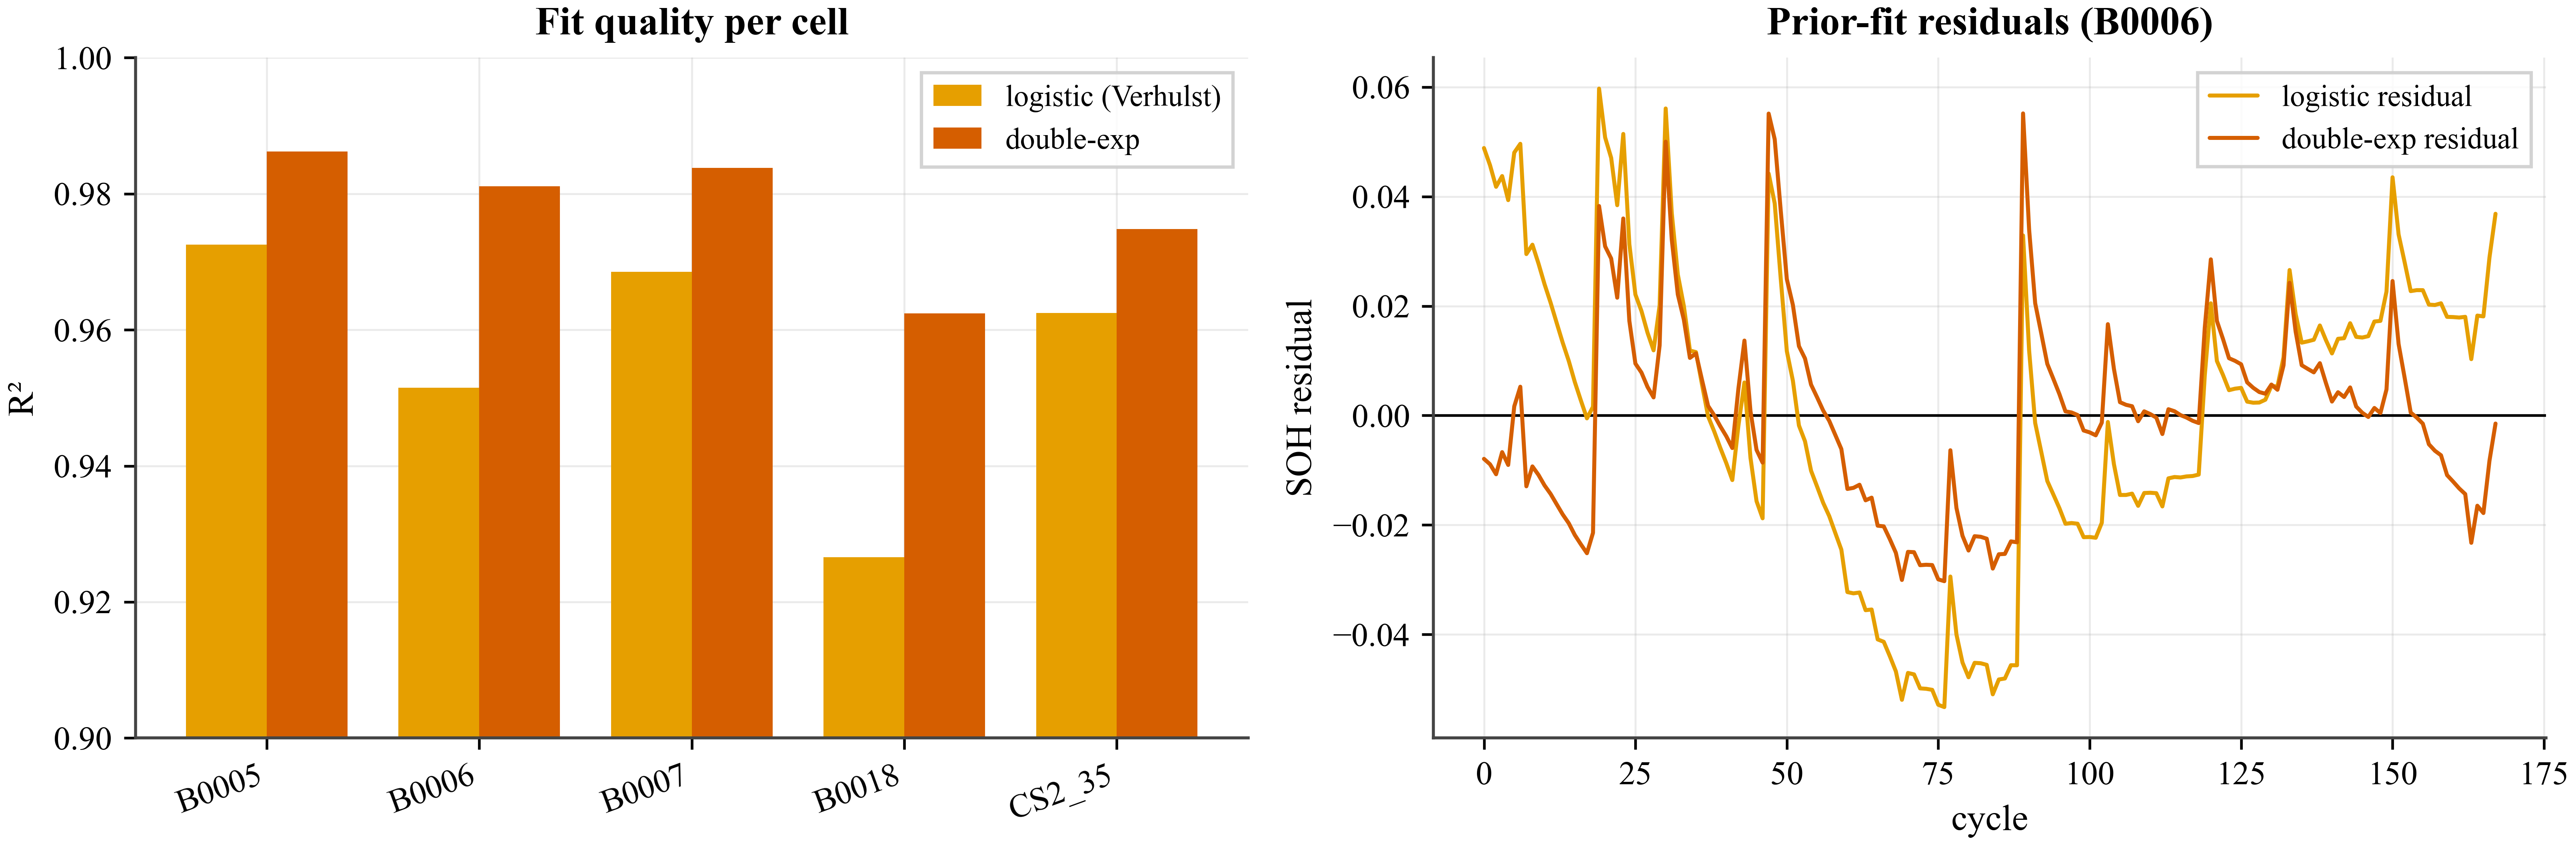
\includegraphics[width=0.95\textwidth]{2-mainmatter/chapters/redundancy.png}
    \caption{Closed-form prior comparison per cell. (Left) the double-exponential
    attains a higher fit quality ($R^2$) than the logistic on every cell; (Right)
    it also produces a smaller residual spread. This justifies retaining the
    two-timescale prior alongside the logistic.}
    \label{fig:redundancy}
\end{figure}

\textbf{(2) A fixed prior cannot describe atypical cells.} Cell B0006 begins
\emph{above} rated capacity (initial SOH $\approx101.8\%$) and exhibits the
heaviest capacity regeneration. Figure~\ref{fig:fit_b0006} shows that even the
flexible double-exponential, when fit to B0006, struggles with its early
super-rated bulge --- and a prior fit on the \emph{other} cells (as required
under LOCO) mismatches B0006 even more. This observation leads to the central
finding of Section~\ref{sec:central_finding}.

\begin{figure}[H]
    \centering
    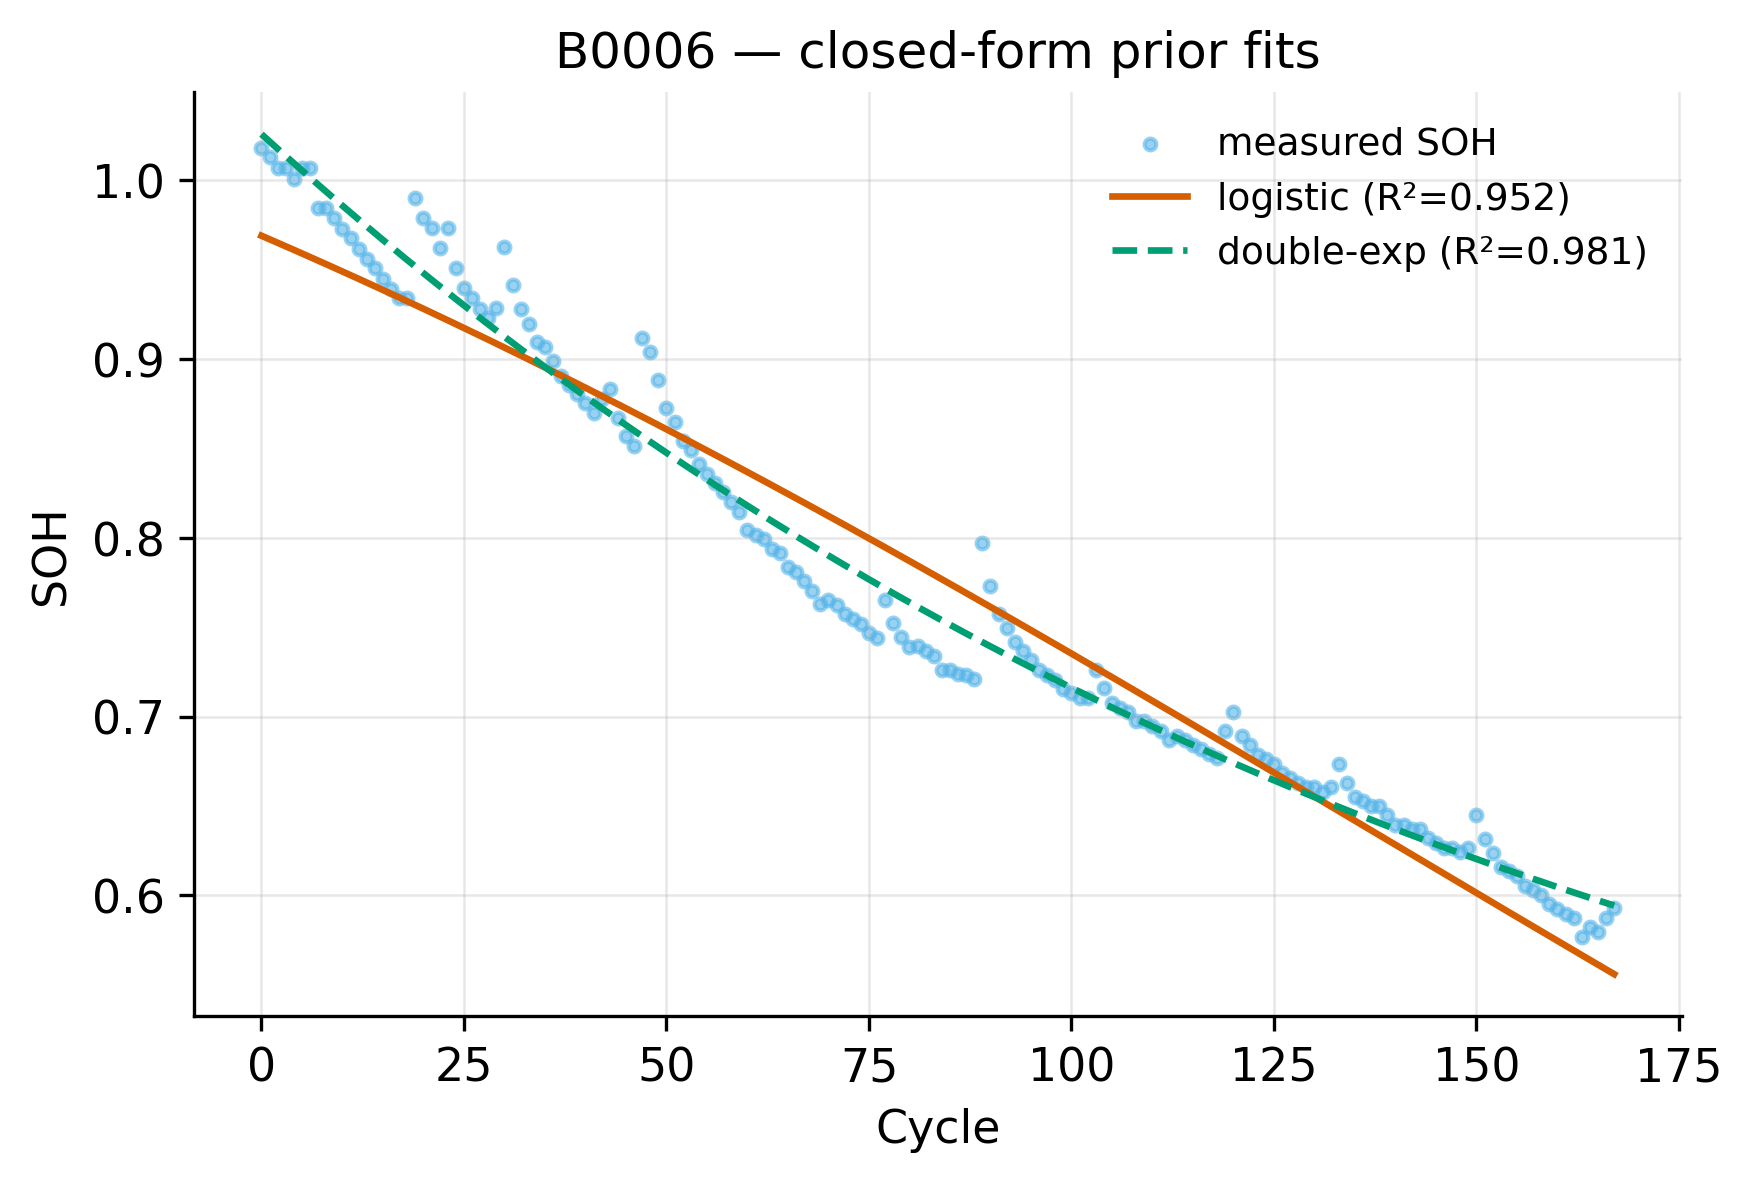
\includegraphics[width=0.85\textwidth]{2-mainmatter/chapters/fit_overlay_B0006.png}
    \caption{Closed-form prior fits for the atypical cell B0006. The cell starts
    above rated capacity and regenerates heavily; the fixed closed-form prior
    (route~A) cannot track this without dragging predictions away from the data.}
    \label{fig:fit_b0006}
\end{figure}

Route~B, in contrast, does not use a fixed curve: it learns its Verhulst
parameters during training. On the held-out folds it converged to
$r\approx-0.87$ and a carrying capacity $K\approx0.91$ (both expressed in the
fixed-scale cycle coordinate, so $r$ is a rate per 500 cycles rather than per
cycle, and its physical interpretation is correspondingly coarser). With a
negative rate constant the logistic law becomes a decay law: for
$\mathrm{SOH} < K$ the learned dynamics give $d\mathrm{SOH}/dt<0$, i.e.\ a
monotone fade whose rate adapts to the training distribution instead of
following a fixed shape. These two learned scalars can be inspected directly, so
the interpretability benefit of the physics prior is retained even though its
parameters are learned.

\section{Main Benchmark (NASA Leave-One-Cell-Out)}
\label{sec:main_benchmark}

Table~\ref{tab:benchmark} and Figures~\ref{fig:benchmark_rmse}--\ref{fig:phys_cons}
summarise the headline comparison across all folds and seeds.

\begin{table}[H]
\centering
\caption{Model benchmark on NASA leave-one-cell-out (measured values; SOH
RMSE as mean $\pm$ 95\% CI). ``Phys.Cons.'' is the fraction of predictions
respecting $d\mathrm{SOH}/dt\le0$; ``Cross'' is the zero-shot NASA$\rightarrow$CALCE RMSE.
The first two rows are the non-learned reference floors of
Chapter~\ref{ch:datasets_implementation} (Table~\ref{tab:benchmarks}). All
learned models receive the same fixed-scale cycle input. The two hybrids use a
deliberately generous hidden size for this comparison; the matched-size
(11k-parameter) deployment model is evaluated separately
(Section~\ref{sec:footprint}).}
\label{tab:benchmark}
\small
\setlength{\tabcolsep}{4.5pt}
\begin{tabular}{l r c c c c}
\toprule
\textbf{Model} & \textbf{Params} & \textbf{SOH RMSE} & \textbf{SOH MAE} & \textbf{Phys.Cons.} & \textbf{Cross RMSE} \\
\midrule
\multicolumn{6}{l}{\emph{Non-learned reference floors}}\\
Double-exp fit     &        4 & $0.0449 \pm 0.0065$ & 0.0397 & 0.995          & 0.6721 \\
SVR                &  6{,}966 & $0.0495 \pm 0.0106$ & 0.0371 & 0.732          & 0.1566 \\
\midrule
\multicolumn{6}{l}{\emph{Learned models}}\\
Transformer (light)  & 17{,}441  & $0.0345 \pm 0.0075$ & 0.0312 & 0.783 & \textbf{0.0859} \\
Transformer (heavy) & 225{,}409 & $0.0418 \pm 0.0084$ & 0.0384 & 0.715 & 0.1018 \\
LSTM               &  5{,}537 & $0.0359 \pm 0.0182$ & 0.0329 & 0.805          & 0.0993 \\
GRU                &  4{,}161 & $0.0359 \pm 0.0088$ & 0.0324 & 0.772          & 0.1125 \\
Neural-ODE         &  \textbf{1{,}249} & $0.0505 \pm 0.0196$ & 0.0450 & 0.686 & 0.0977 \\
\textbf{Hybrid (route B)} & 41{,}473 & $\mathbf{0.0262 \pm 0.0029}$ & \textbf{0.0216} & \textbf{0.918} & 0.2617 \\
Hybrid (route A)   & 41{,}473 & $0.0301 \pm 0.0059$ & 0.0258 & 0.903          & 0.0963 \\
\bottomrule
\end{tabular}
\end{table}

\begin{figure}[H]
    \centering
    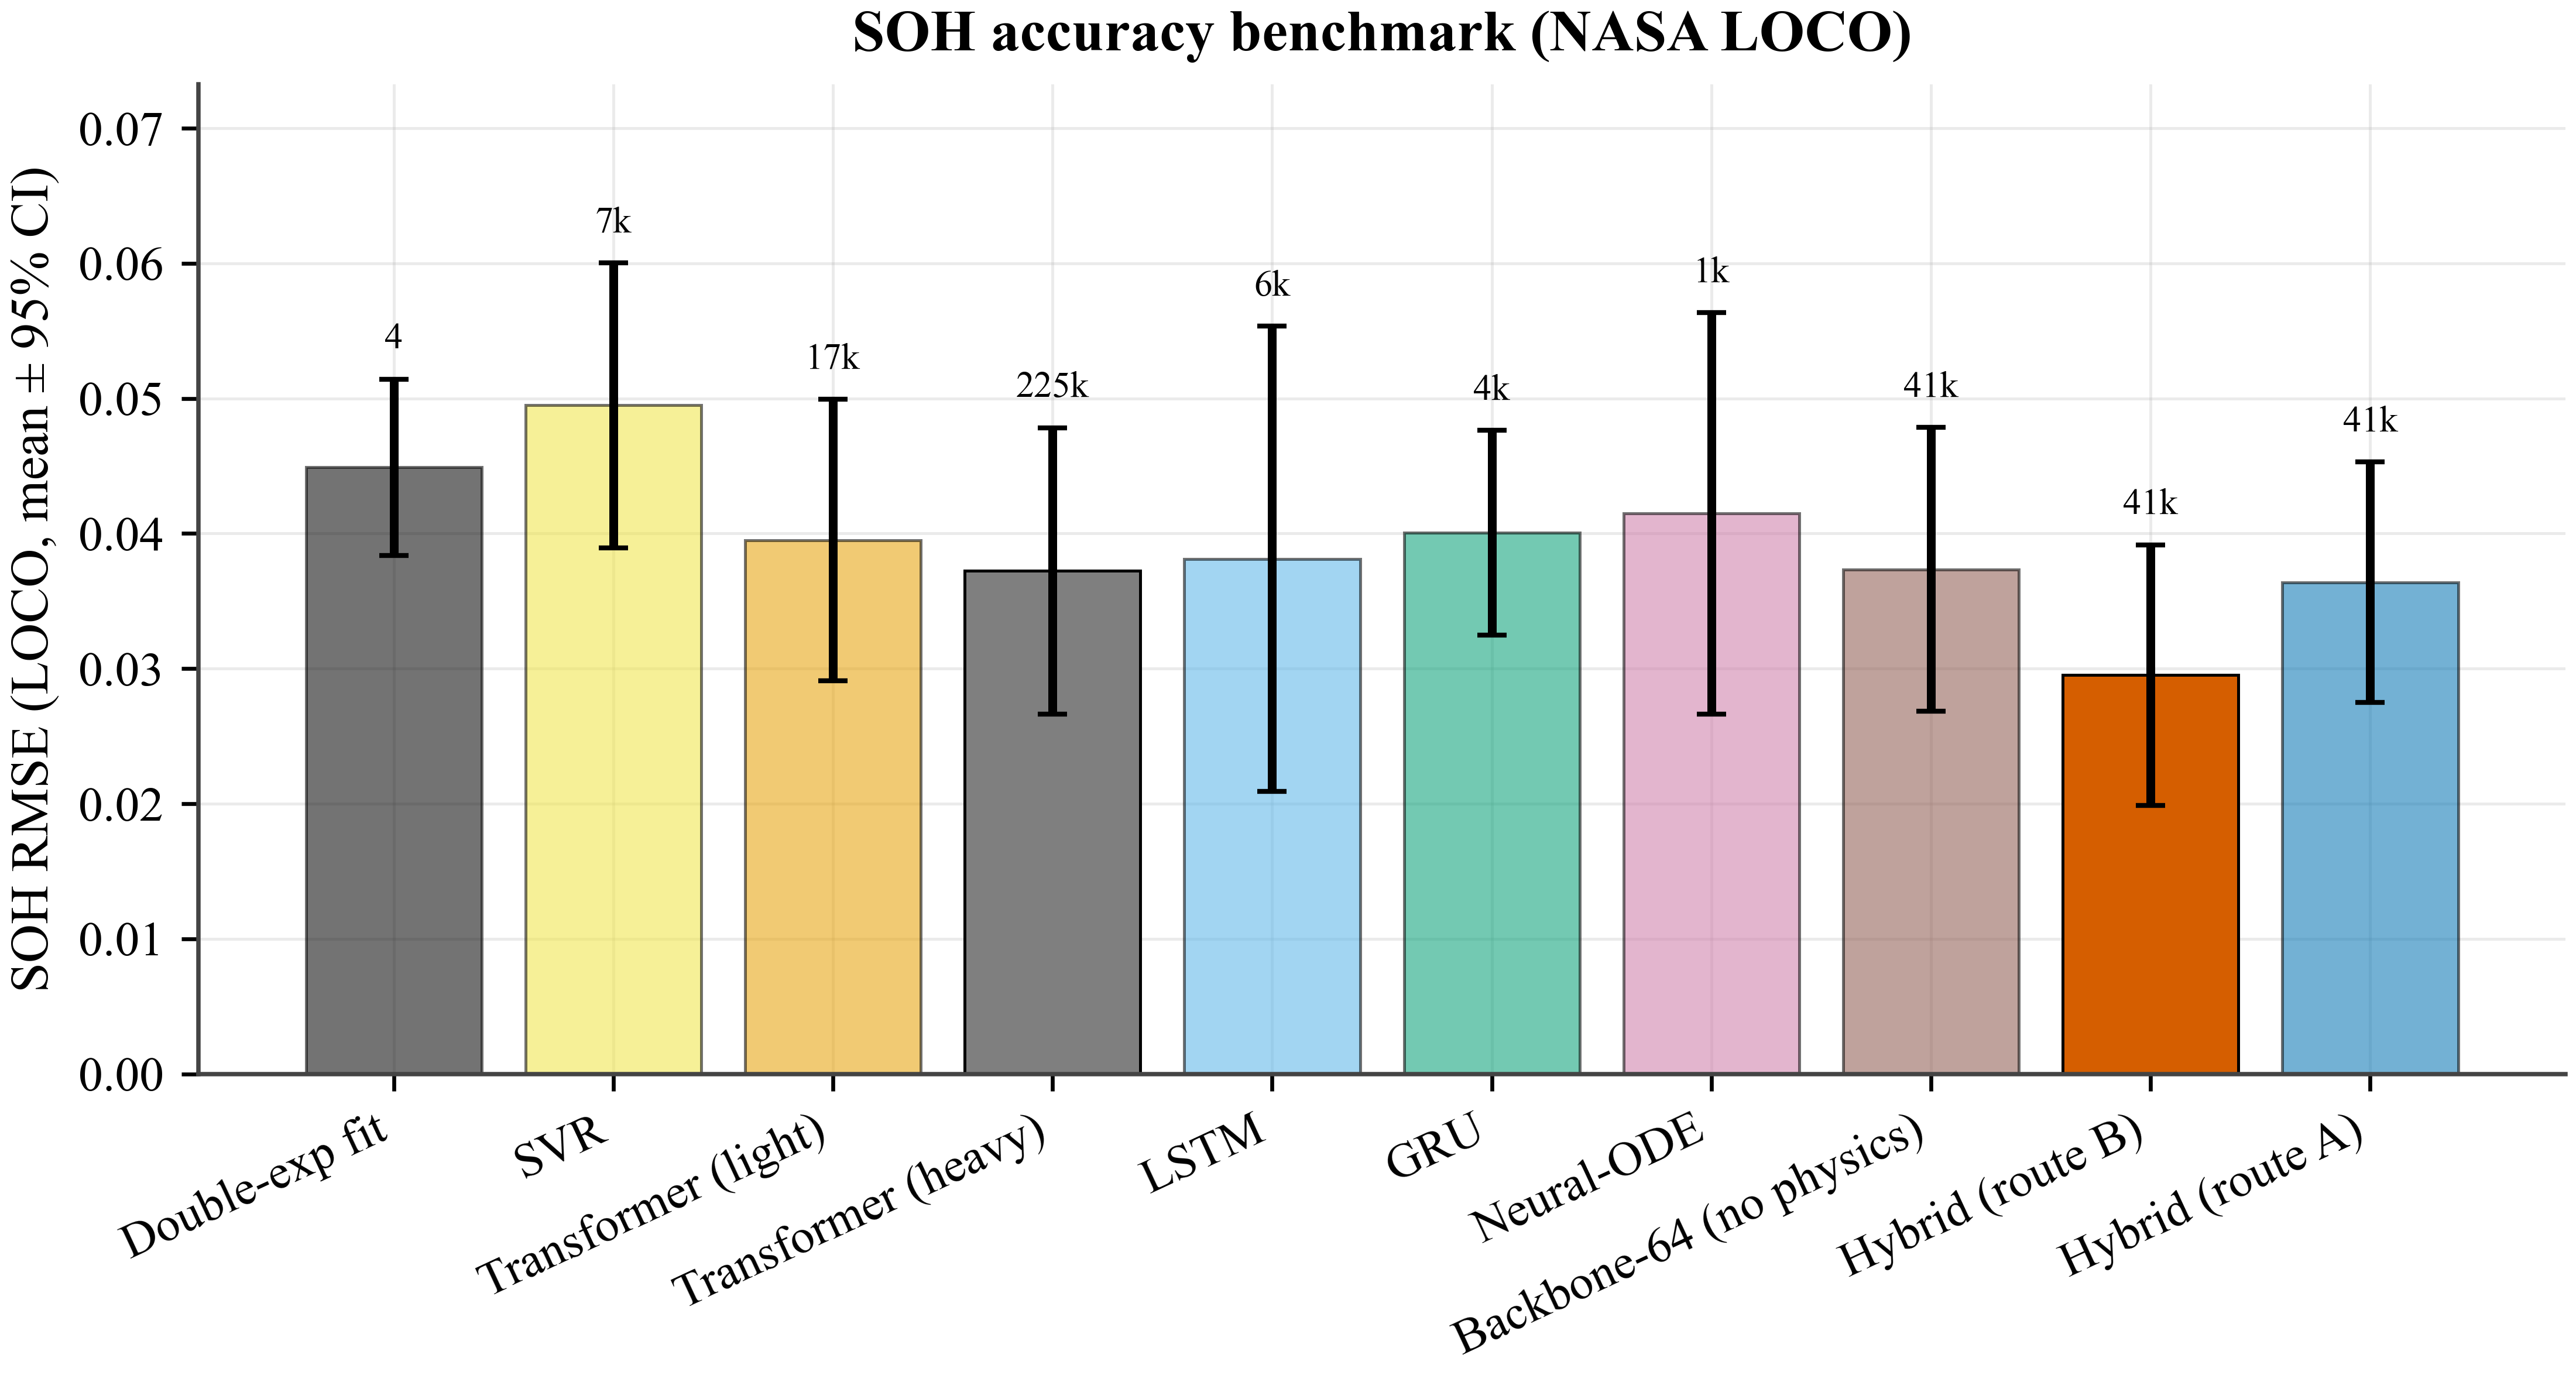
\includegraphics[width=0.85\textwidth]{2-mainmatter/chapters/benchmark_rmse_bar.png}
    \caption{SOH RMSE on NASA leave-one-cell-out (mean $\pm$ 95\% CI; parameter
    counts above the bars). The route-B hybrid attains the lowest mean RMSE and
    the narrowest confidence interval; the 13$\times$ larger heavy Transformer is
    less accurate than the light one.}
    \label{fig:benchmark_rmse}
\end{figure}

\begin{figure}[H]
    \centering
    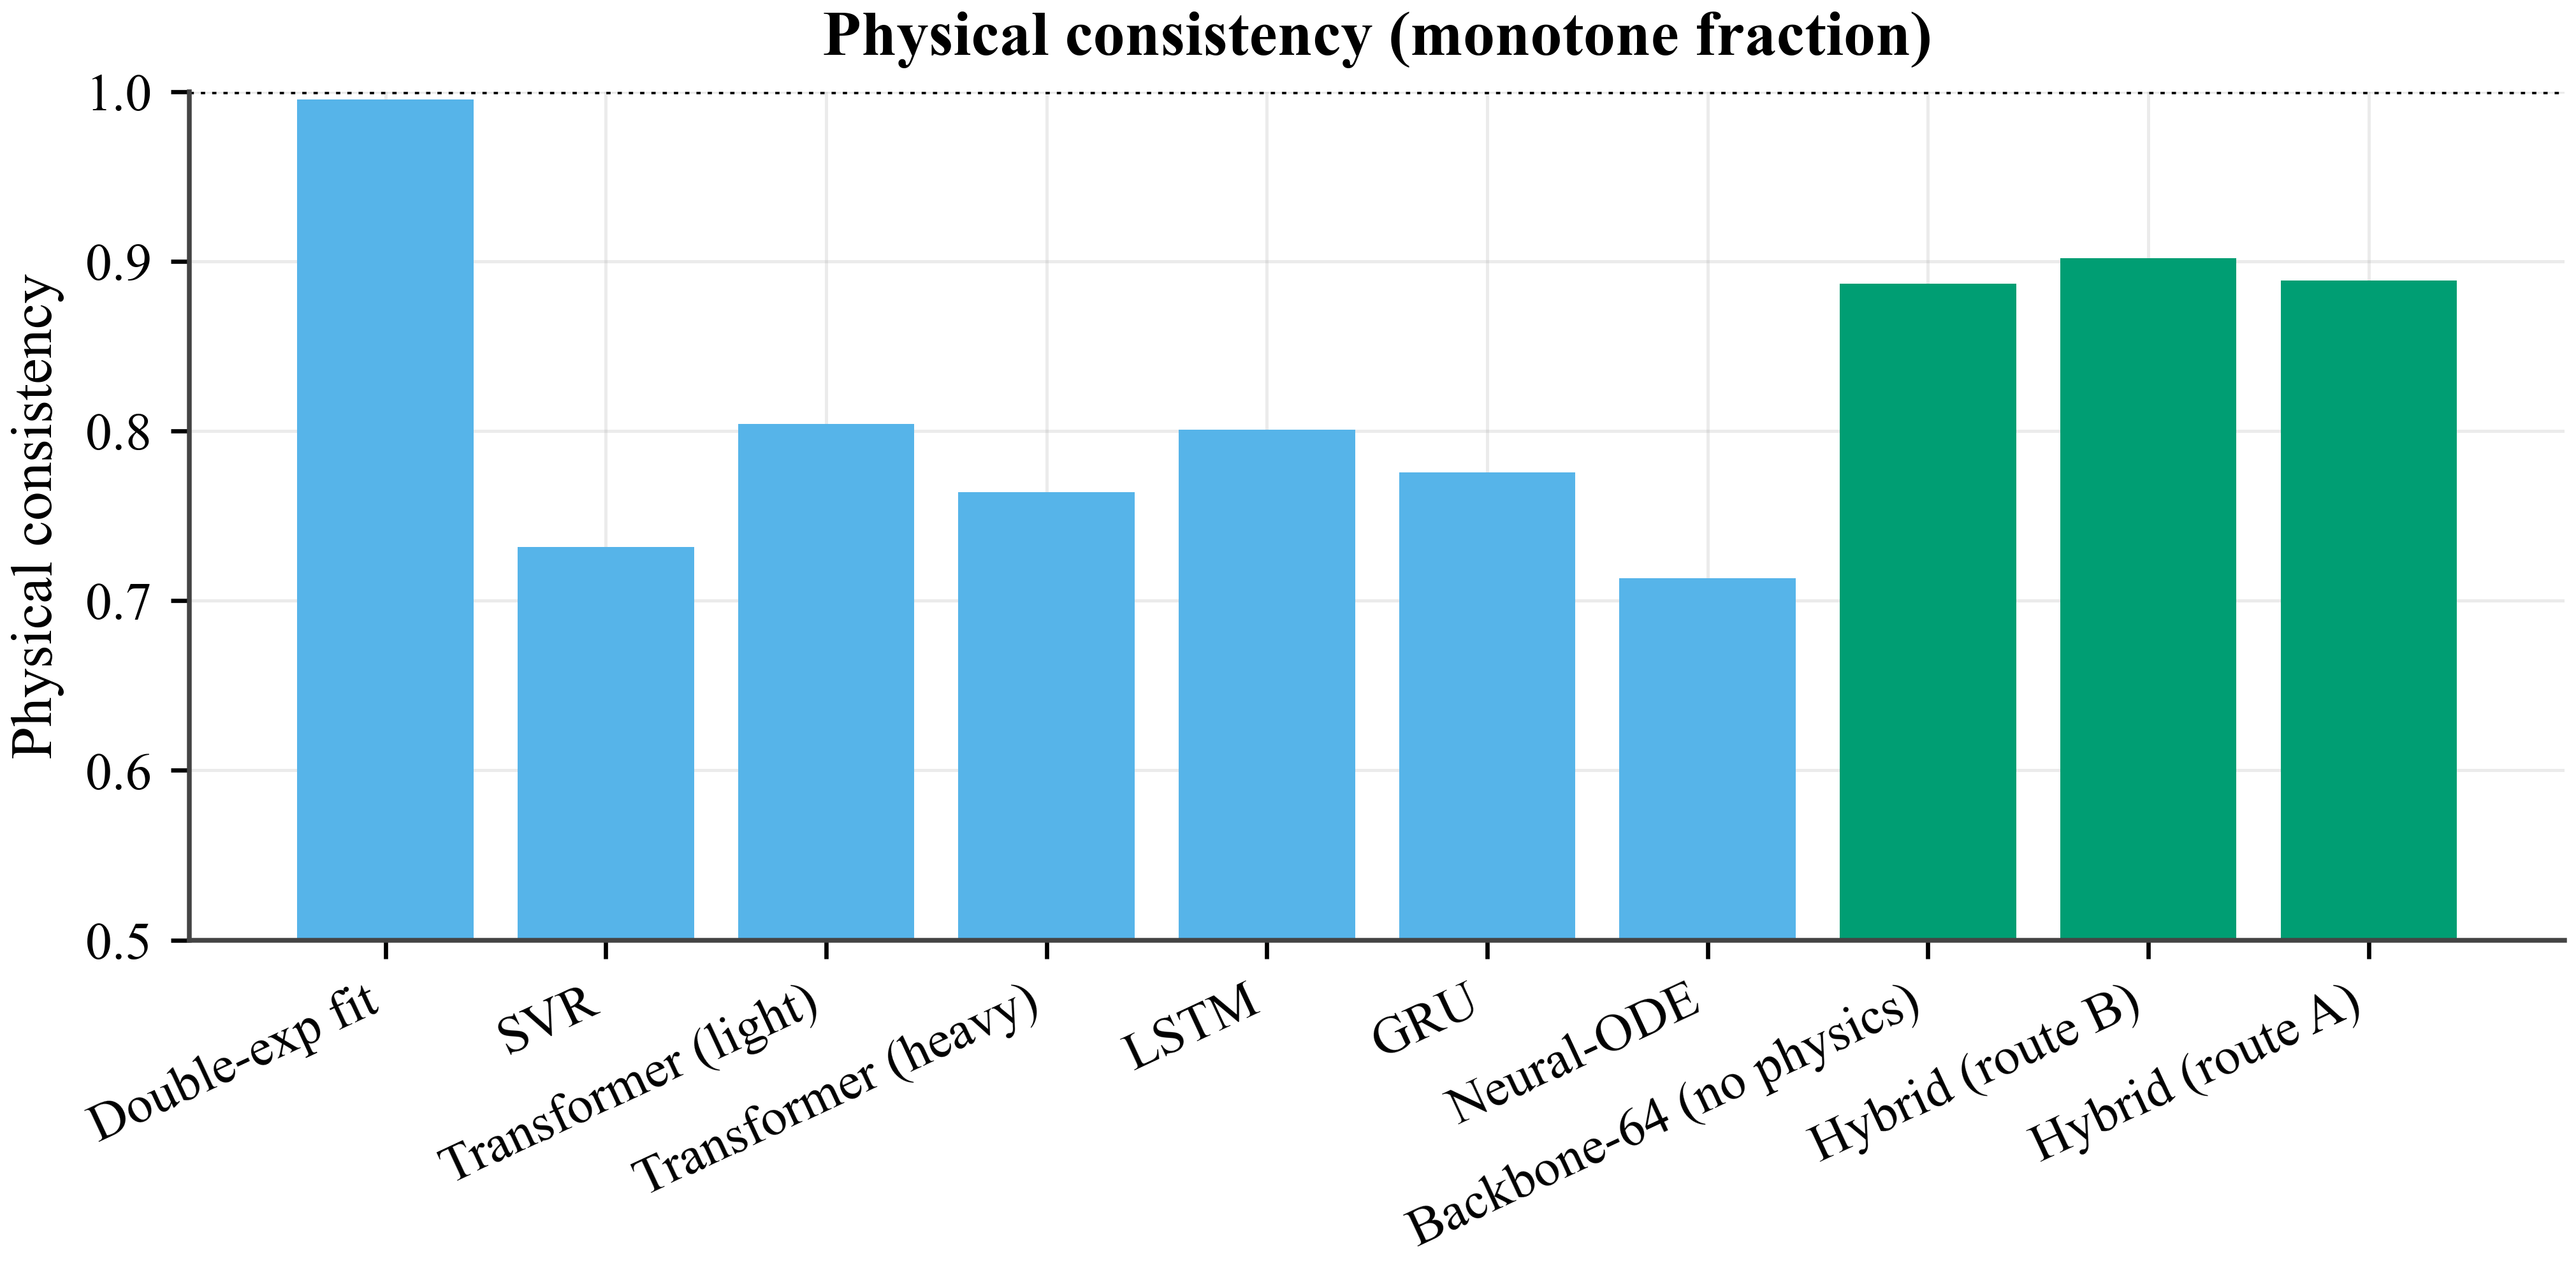
\includegraphics[width=0.85\textwidth]{2-mainmatter/chapters/phys_consistency_bar.png}
    \caption{Physical plausibility (fraction of predictions with
    $d\mathrm{SOH}/dt\le0$). The route-B hybrid is the most physically consistent
    \emph{learned} model (0.918), well above all purely data-driven baselines. Two
    reference points bound the metric: the double-exponential curve fit scores
    0.995 only trivially (a fitted closed-form curve is monotone by construction),
    and the ground-truth SOH itself scores 0.85--0.90 on the NASA cells because of
    genuine regeneration. Route~B's score above the ground-truth reference means
    it smooths through some real regeneration transients; the metric is read as
    trend plausibility, not as accuracy.}
    \label{fig:phys_cons}
\end{figure}

Several observations follow from Table~\ref{tab:benchmark}:

\begin{itemize}
    \item \textbf{The route-B hybrid is the most accurate model} on unseen NASA
    cells (RMSE $0.0262 \pm 0.0029$), with the narrowest confidence interval of
    any model, ahead of the light Transformer ($0.0345$) and the LSTM/GRU
    ($0.0359$). It is also the most physically consistent learned model
    ($0.918$ vs.\ $0.805$ for the LSTM).
    \item \textbf{Most learned models clear the empirical floors; one does not.}
    The double-exponential curve fit reaches $0.0449$ and the SVR $0.0495$ on
    held-out cells. All recurrent, attention and hybrid models beat both floors.
    The Neural-ODE ($0.0505$) does \emph{not}: encoding only the final window
    step and integrating a learned latent field is too weak for this task, and
    this is reported plainly rather than hidden. The curve fit also transfers
    poorly (Cross RMSE $0.67$ on the 878-cycle CALCE cell), and its near-perfect
    physical consistency ($0.995$) carries little information, since a fitted
    closed-form curve is monotone by construction.
    \item \textbf{Attention capacity does not pay at this data scale.} The
    edge-sized light Transformer reaches $0.0345$, and the 13$\times$ larger
    heavy model is worse, at $0.0418$. Section~\ref{sec:transformer_gap}
    quantifies the comparison against the hybrid.
    \item \textbf{The LSTM's mean hides a failure mode.} Its wide interval
    ($\pm0.0182$) is driven by the atypical cell B0006, where its per-cell RMSE
    degrades to $0.068$ (Table~\ref{tab:perfold}) --- the same atypical-cell
    weakness the fixed prior shows, discussed next.
    \item \textbf{Cross-dataset transfer is led by the light Transformer}
    ($0.0859$), with route~A ($0.0963$), Neural-ODE ($0.0977$), LSTM ($0.0993$)
    and the heavy Transformer ($0.1018$) close behind. \textbf{Route~B degrades
    to $0.2617$} out of distribution --- an honest negative result analysed in
    Section~\ref{sec:transformer_gap}: its learned dynamics depend on the cycle
    coordinate, which extrapolates far outside the training range on the
    long-lived CALCE cell. Only one CALCE test cell is available, so all
    cross-dataset numbers are indicative.
\end{itemize}

\section{The Central Finding: Learnable Physics (Route B) Outperforms the Fixed Prior}
\label{sec:central_finding}

The most important comparison in this thesis is between the two physics
mechanisms, with the strongest purely data-driven baseline (the LSTM) alongside.
Table~\ref{tab:perfold} breaks the result down per test cell.

\begin{table}[H]
\centering
\caption{Per-cell SOH RMSE (mean over 3 seeds) under leave-one-cell-out. The
learnable route~B is best or near-best on every cell; the fixed prior (route~A)
trails it on the atypical cells; the purely data-driven LSTM fails on the
atypical B0006.}
\label{tab:perfold}
\begin{tabularx}{0.85\textwidth}{@{} l *{4}{>{\centering\arraybackslash}X} @{}}
\toprule
\textbf{Test cell} & \textbf{B0005} & \textbf{B0006} & \textbf{B0007} & \textbf{B0018} \\
\midrule
Hybrid (route A) & 0.037 & 0.036 & \textbf{0.023} & 0.025 \\
Hybrid (route B) & \textbf{0.030} & \textbf{0.029} & 0.024 & \textbf{0.021} \\
LSTM             & 0.032 & 0.068 & \textbf{0.021} & 0.023 \\
\bottomrule
\end{tabularx}
\end{table}

Three observations follow. First, \textbf{route~B is best or within $0.003$ of
best on every cell} ($0.021$--$0.030$), which is the uniformity a fleet BMS
needs on cells it has never seen. Second, \textbf{route~A trails route~B
consistently and most on the atypical cells} (B0005, B0006 --- the cells whose
trajectories a prior fit on other cells does not describe;
Figure~\ref{fig:fit_b0006}); after correcting a coordinate mismatch in the
prior evaluation found during code review, route~A no longer fails
catastrophically, but the learnable mechanism remains better everywhere except
B0007. Third, \textbf{the purely data-driven LSTM fails exactly where the fixed
prior struggles}: on B0006 (starts above rated capacity, heaviest regeneration)
its error doubles to $0.068$. Both a rigid prior and pure data-driving are
weakest on cells unlike the training population; the learnable physics residual
is the only variant that stays uniform. Figure~\ref{fig:soh_b0005} shows the
held-out predictions on B0005.

\begin{figure}[H]
    \centering
    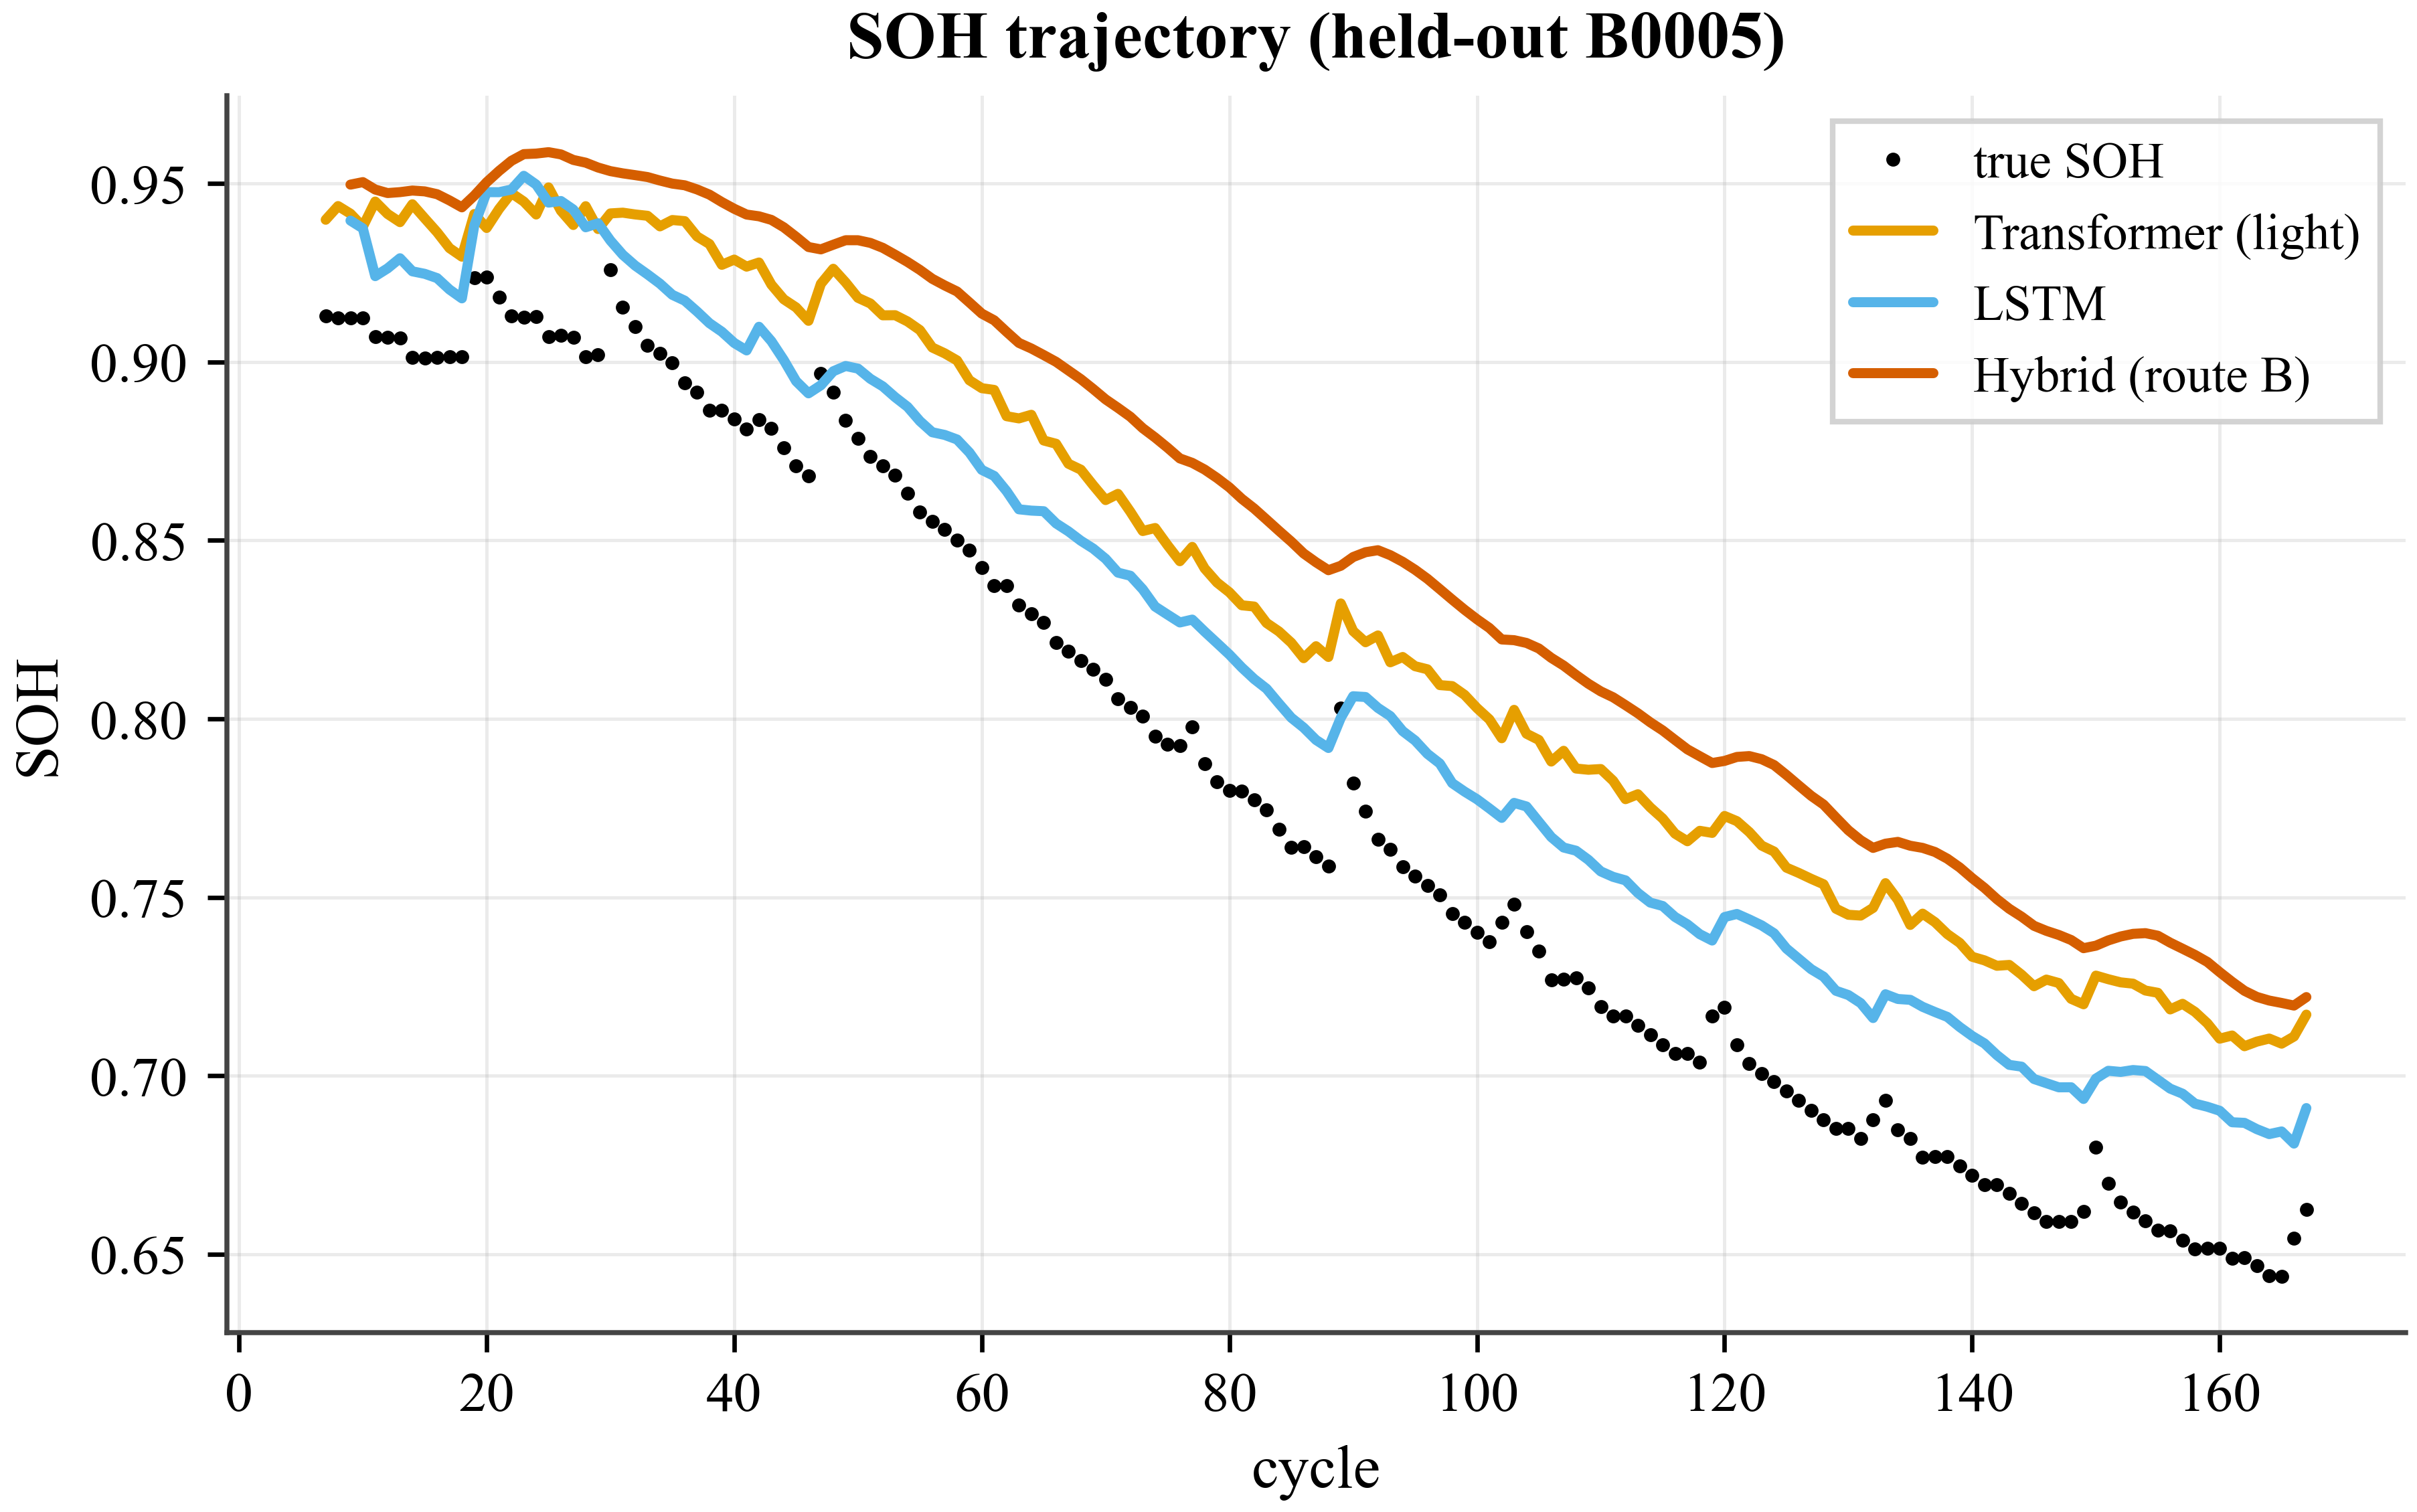
\includegraphics[width=0.85\textwidth]{2-mainmatter/chapters/soh_overlay_B0005.png}
    \caption{SOH trajectory on the held-out cell B0005. Models trained on the
    other cells tend to over-estimate SOH as the real capacity fades faster than
    the training population suggests; over-estimation is the dangerous direction
    for a BMS, since it makes the cell look healthier than it is. The hybrid
    stays closest to the measured curve.}
    \label{fig:soh_b0005}
\end{figure}

\paragraph{Summary.} The lightweight physics-informed approach holds, and the
physics mechanism matters: the learnable ODE-residual (route~B) should be
preferred over the fixed closed-form prior (route~A). Route~B costs roughly
$2$--$3\times$ more training time (Section~\ref{sec:ablations}) in exchange for
uniform accuracy across cells and the best physical plausibility. Since training
is performed offline, this is an acceptable trade for a safety-critical
application.

\section{The Transformer Question: Heavy Attention Does Not Pay on Scarce Data}
\label{sec:transformer_gap}

Chapters 1 and 2 motivated this work with the observation that attention models
lead the literature on accuracy but are too heavy for standard BMS hardware, so a
lightweight physics-informed model should aim to match their accuracy at a
fraction of the footprint. The measured results support a stronger statement: at
realistic data volumes, the high-capacity Transformer is not more accurate
either. Transformer results in the literature (e.g.\ SGEformer) are obtained on
large training corpora, whereas run-to-failure data at that scale is rarely
available for a given cell design.

\subsection{The Paired Gap}

Table~\ref{tab:gap} reports the paired comparison against the heavy
Transformer. The test is performed at the fold level ($n=12$ leave-one-cell-out
experiments $=4$ cells $\times$ 3 seeds), which is the appropriate unit of
replication: per-cycle predictions within a cell are strongly autocorrelated, so
pairing thousands of them (as an earlier version of this analysis did) inflates
the effective sample size and yields a meaningless $p\approx5\times10^{-94}$. In
addition, because the models use different sequence lengths, those per-cycle
pairs were not aligned to the same cycles.

\begin{table}[H]
\centering
\caption{Hybrid vs.\ the heavy Transformer, paired at the \emph{fold}
level ($n=12$), with the paired Wilcoxon signed-rank test.}
\label{tab:gap}
\small
\setlength{\tabcolsep}{4pt}
\begin{tabular}{l c c c c c c}
\toprule
\textbf{Comparison} & \textbf{Mean} & \textbf{Transf.} & \textbf{Rel.\ gap} & \textbf{Folds won} & \textbf{Wilcoxon $p$} & \textbf{Sig.} \\
\midrule
Route A vs.\ Transf.\ (SOH RMSE) & 0.0301 & 0.0418 & $-28.0\%$ & 10/12 & 0.012 & yes \\
Route B vs.\ Transf.\ (SOH RMSE) & 0.0262 & 0.0418 & $\mathbf{-37.5\%}$ & 11/12 & 0.007 & yes \\
Route B vs.\ Transf.\ (Phys.\ cons.) & 0.918 & 0.715 & $+28.5\%$ & \textbf{12/12} & $\mathbf{4.9\!\times\!10^{-4}}$ & yes \\
\bottomrule
\end{tabular}
\end{table}

On the in-distribution leave-one-cell-out task the route-B hybrid has a lower
mean SOH RMSE than the heavy Transformer ($-37.5\%$, winning 11 of 12 runs,
run-level $p=0.007$), and is more physically consistent on all 12 runs
(run-level $p\approx5\times10^{-4}$). A statistical caution applies to both
tests: the three seeds within a fold share the same test cell and are therefore
correlated, so $n=12$ overstates the number of independent observations. With
the four cells as the independent unit, the smallest attainable two-sided
Wilcoxon $p$ is $0.125$, so formal significance cannot be established from this
dataset; the defensible statement is descriptive --- \emph{the hybrid is more
accurate and more physically plausible than the heavy Transformer on every cell
(4/4 after seed-averaging) and on nearly every run}.
Figure~\ref{fig:differential} shows the per-cycle differential error on B0018:
positive values mean the hybrid is closer to the ground truth, and the hybrid
stays ahead over the second half of the cell's life as it approaches
end-of-life.

\begin{figure}[H]
    \centering
    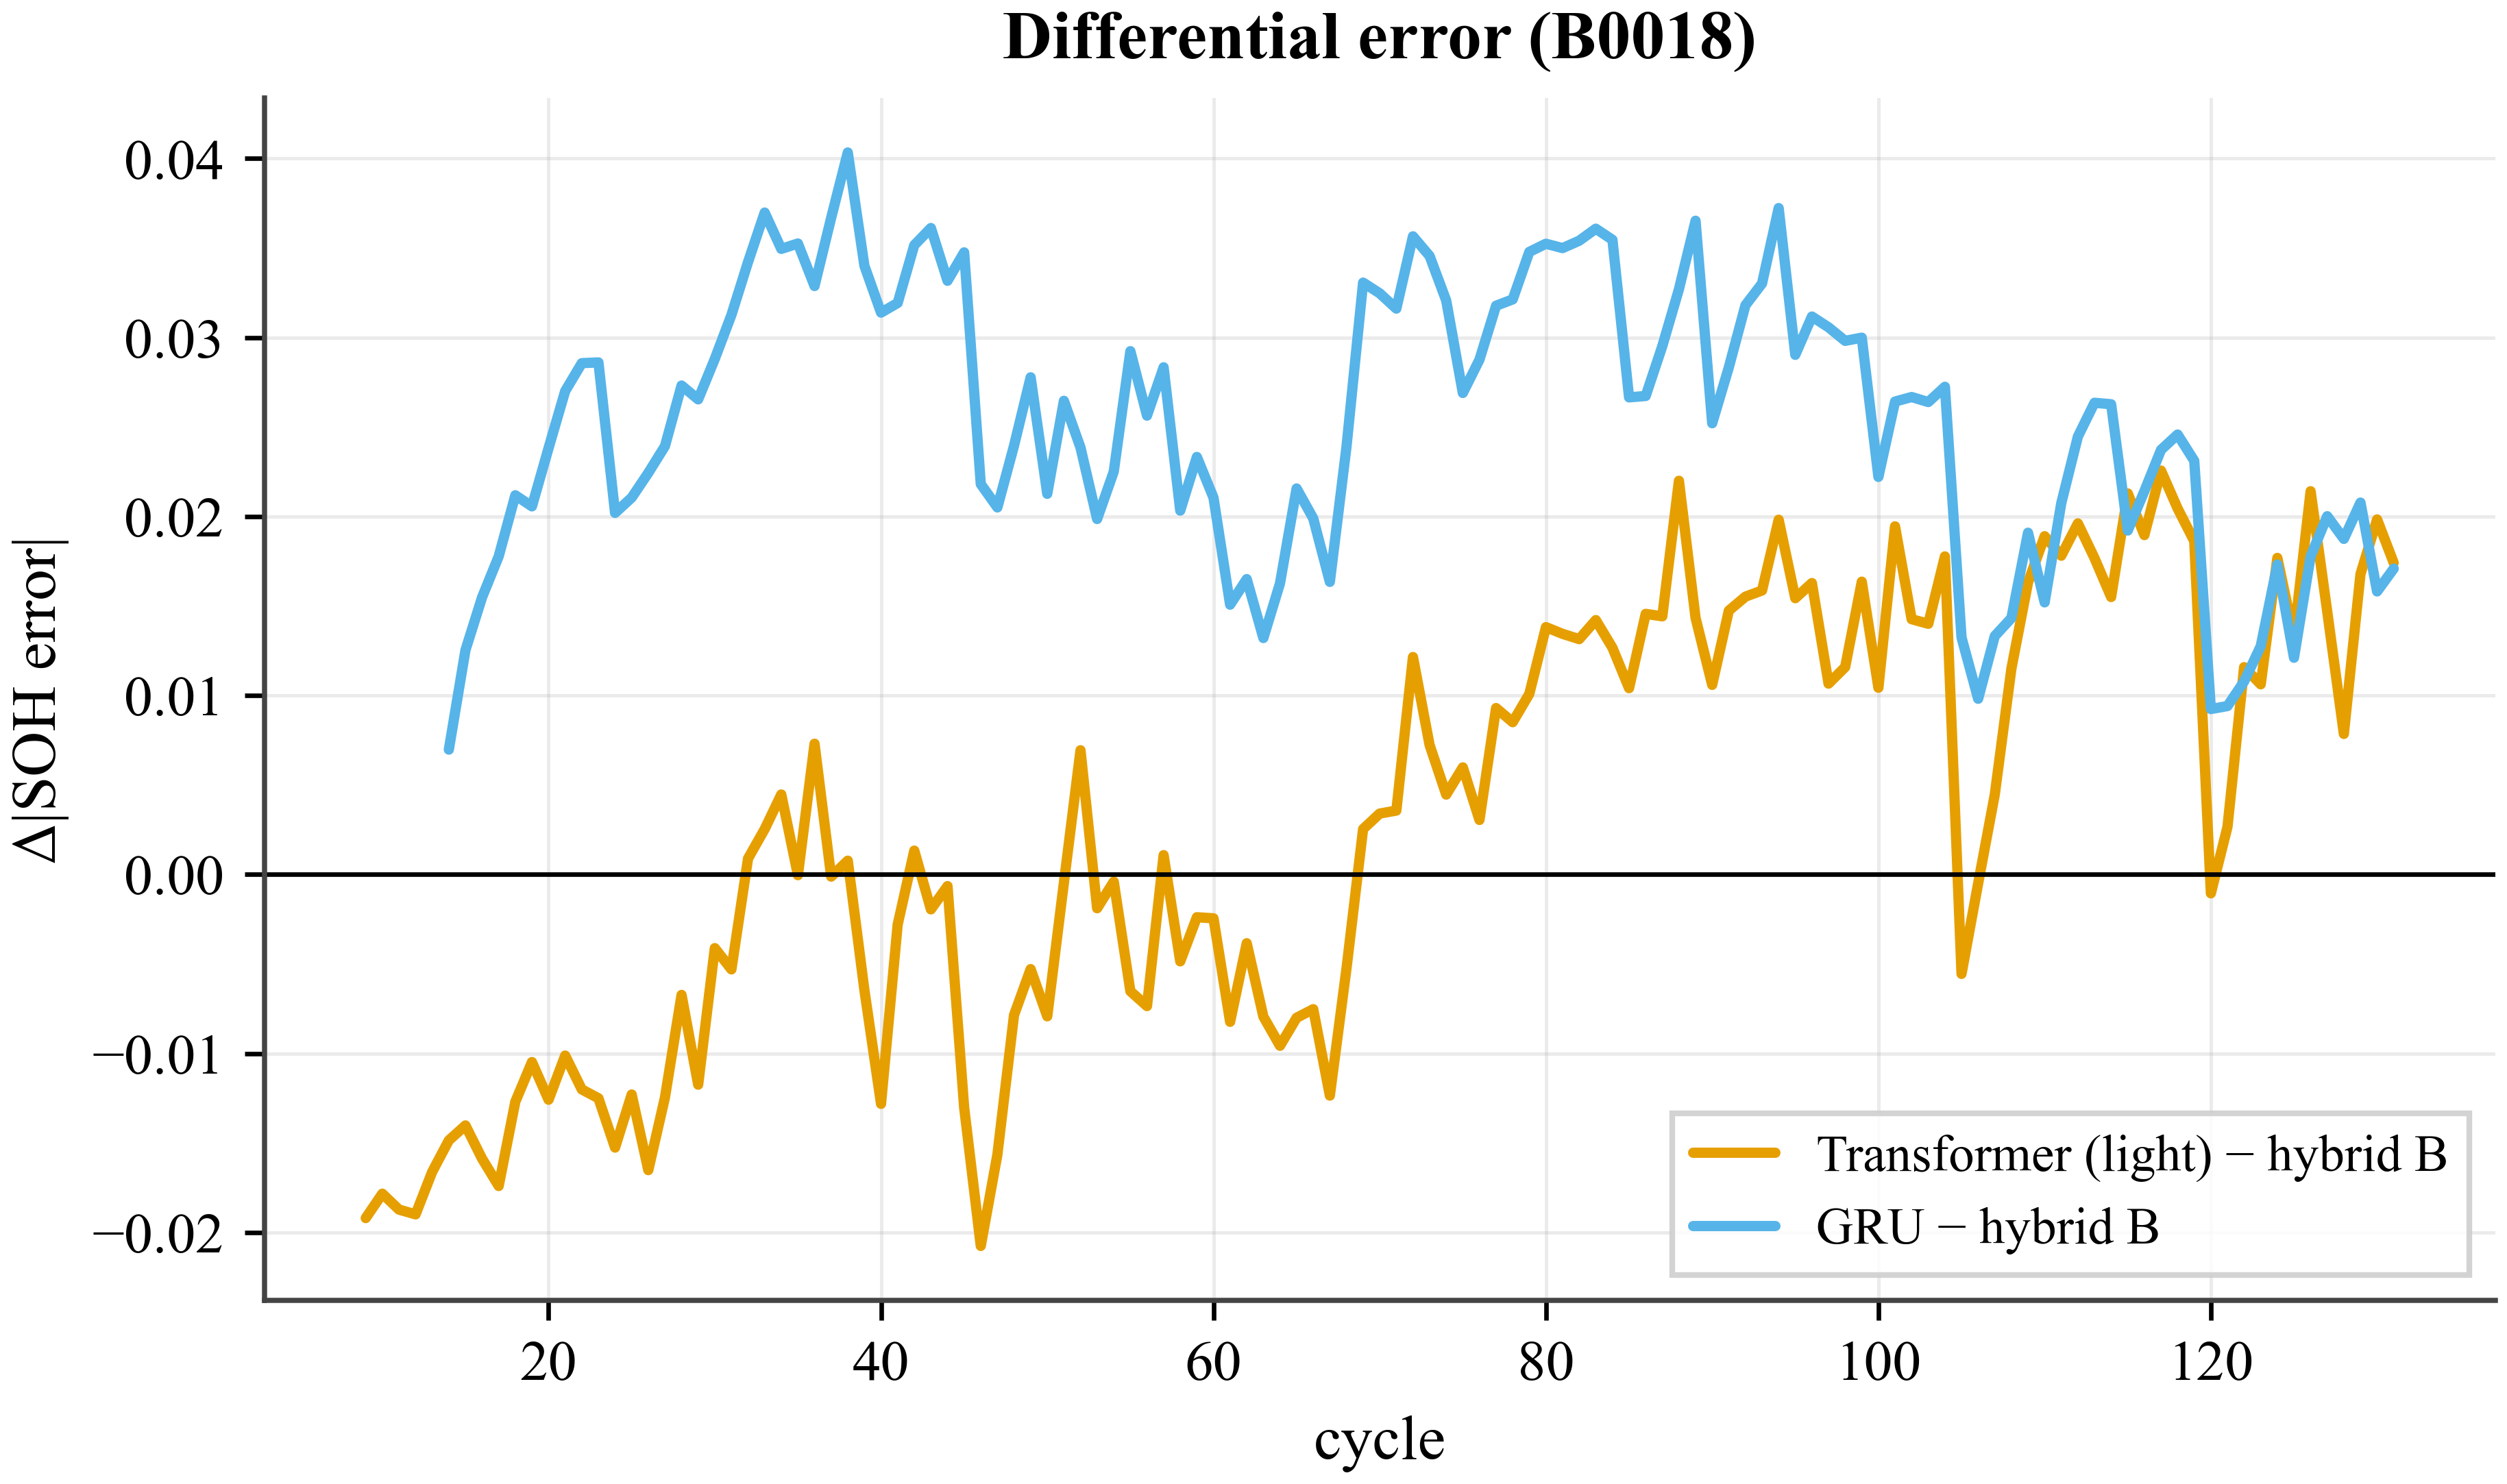
\includegraphics[width=0.85\textwidth]{2-mainmatter/chapters/differential_B0018.png}
    \caption{Differential error plot on B0018: per-cycle $\Delta|\mathrm{SOH}\
    \mathrm{error}|$ (baseline $-$ hybrid). Values above zero indicate the hybrid
    is closer to ground truth than the baseline at that cycle.}
    \label{fig:differential}
\end{figure}

\subsection{Capacity, Scarcity and Overfitting}
\label{sec:overfitting}

Scaling the Transformer from 17k to 225k parameters (13$\times$) makes its
held-out accuracy worse ($0.0345 \rightarrow 0.0418$) despite strong
regularisation (dropout 0.3, weight decay, a longer schedule), which indicates
that the available data cannot constrain the additional capacity. Two stress
tests probe this further (Figure~\ref{fig:scarcity}): a data-volume sweep
(10--100\% of the training cycles) and a train--test generalisation-gap
comparison at full data. Both are run on a reduced protocol (2 folds $\times$
2 seeds) and turn out to be \textbf{noise-dominated at this scale}: no model
shows a clean monotonic trend across data fractions, and the gap estimates are
small relative to their variability (the Transformers' gaps are near zero or
negative on this run, the route-A hybrid's is $+0.007$). These sweeps are
therefore reported as inconclusive rather than as evidence; the reliable,
full-protocol evidence for the capacity conclusion is the main benchmark itself
(13$\times$ more attention parameters produced a \emph{less} accurate, less
physically consistent, worse-calibrated model), together with the footprint cost
of that capacity (Section~\ref{sec:footprint}).

\begin{figure}[H]
    \centering
    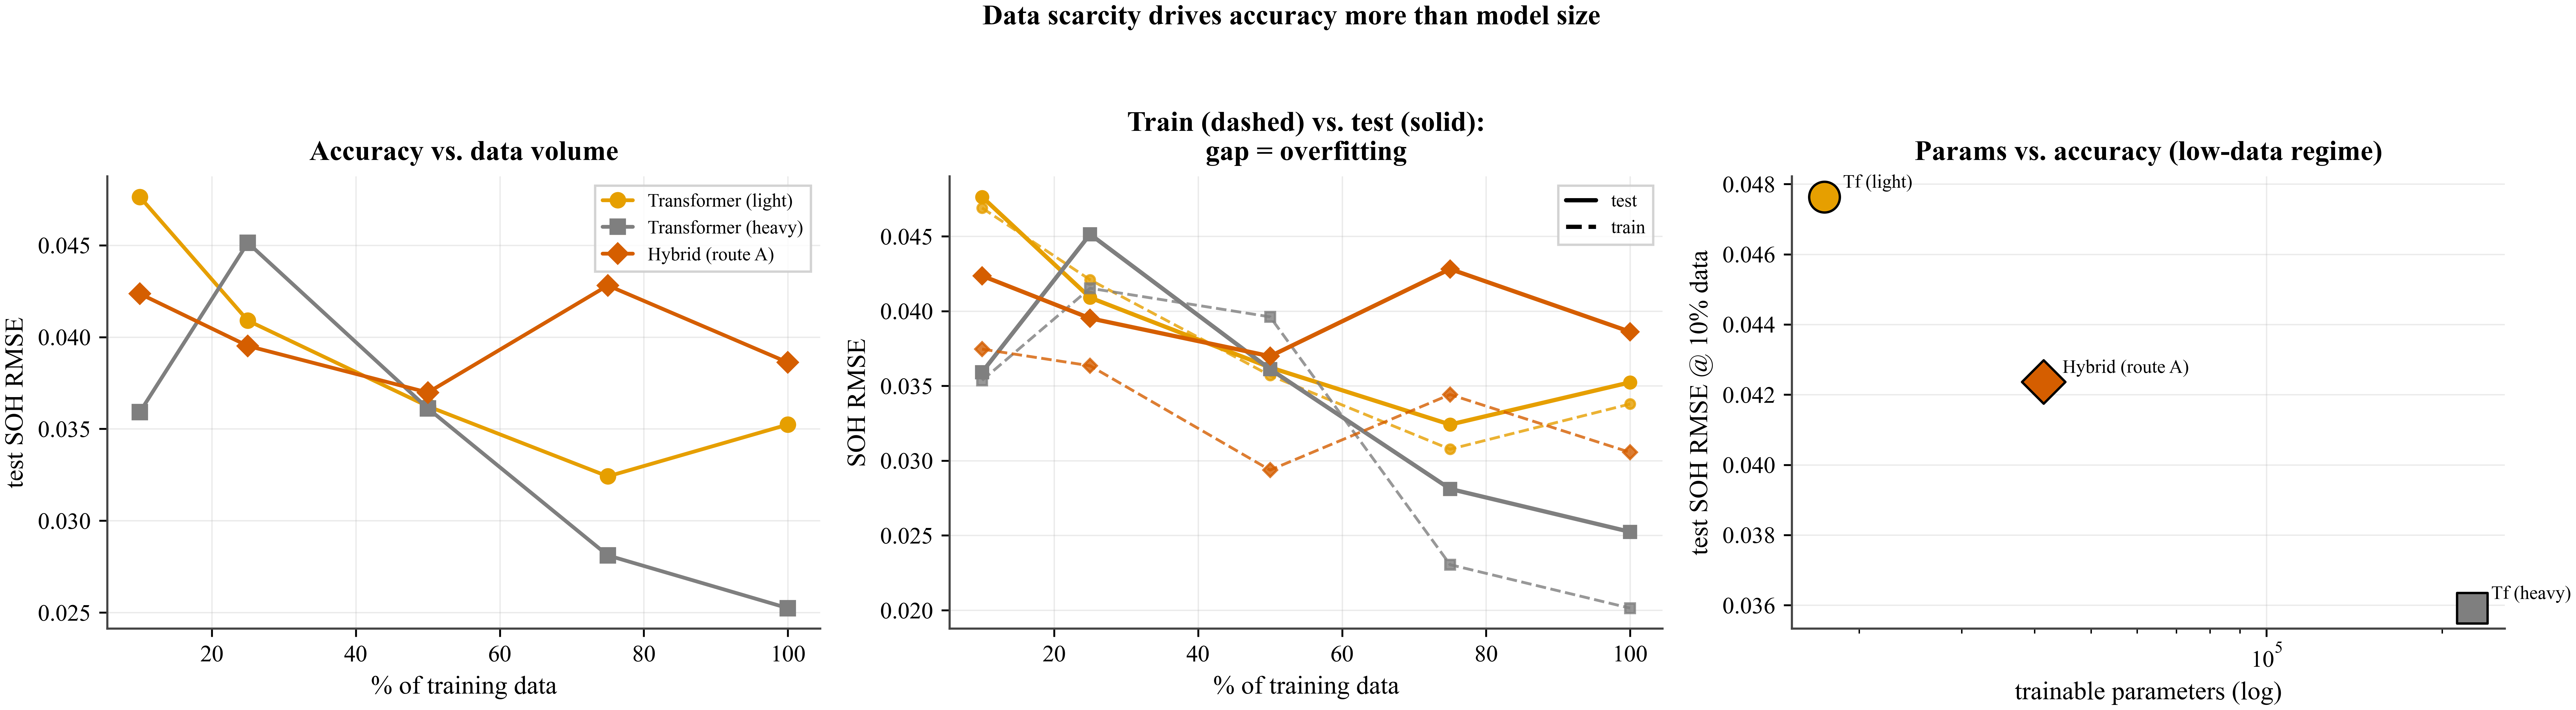
\includegraphics[width=1.0\textwidth]{2-mainmatter/chapters/scarcity_stress_test.png}
    \caption{Data-volume stress test (2 folds $\times$ 2 seeds; indicative).
    (Left) test RMSE vs.\ training-data fraction; (Middle) train vs.\ test
    curves; (Right) parameters vs.\ accuracy in the low-data regime. At this
    reduced protocol the sweeps are noise-dominated and no clean trend survives;
    the capacity conclusion in the text rests on the full four-fold benchmark
    instead.}
    \label{fig:scarcity}
\end{figure}

\subsection{Cross-Dataset Transfer and an Honest Negative Result}
\label{sec:cross_dataset}

On the zero-shot NASA$\rightarrow$CALCE transfer the light Transformer leads
($0.0859$), with route~A, the Neural-ODE, the LSTM and the heavy Transformer
between $0.096$ and $0.102$, and the plain GRU at $0.113$. \textbf{Route~B
degrades to $0.2617$ --- the worst learned model out of distribution.} The
mechanism is the cycle coordinate: CALCE CS2\_35 lives for 878 cycles, so the
fixed-scale coordinate reaches $1.76$ at end-of-test, far outside the training
range ($\le0.34$ on the NASA cells), and route~B's learned dynamics --- which
depend on that coordinate through the ODE residual --- extrapolate poorly.
(Under the earlier, leaked normalization every test trajectory was rescaled into
$[0,1]$, which masked exactly this failure; the corrected protocol exposes it.)
Two mitigations are identified for future work: saturating the coordinate at the
training maximum, and running the deployed zeroed-coordinate path (which the
footprint profiling already uses) for out-of-range cells. With only a single
CALCE test cell, all cross-dataset rankings remain indicative; the in-distribution
LOCO results are the load-bearing evidence of this thesis.

\section{Prognostic (PHM) Assessment}
\label{sec:phm}

Beyond pointwise SOH error, the models were assessed with standard Prognostics and
Health Management metrics: the $\alpha$-$\lambda$ accuracy (fraction of the life
within a $\pm20\%$ cone of true RUL), Prognostic Horizon (PH), and Cumulative
Relative Accuracy (CRA). RUL is derived from the predicted SOH trajectory and the
EOL threshold (standard PHM practice), not a separate regressor.

\begin{table}[H]
\centering
\caption{Prognostic (PHM) metrics on NASA leave-one-cell-out (mean over
folds$\times$seeds). CRA punishes early-life over- and under-shoot; negative CRA
indicates badly calibrated early-life horizons.}
\label{tab:phm}
\small
\begin{tabular}{l c c c}
\toprule
\textbf{Model} & \textbf{$\alpha$-$\lambda$ accuracy} & \textbf{Prognostic horizon} & \textbf{CRA} \\
\midrule
Double-exp fit        & 0.72 & 83.3 & 0.37 \\
SVR                   & 0.72 & 82.8 & 0.48 \\
Transformer (light)   & 0.62 & 77.8 & 0.11 \\
Transformer (heavy)   & 0.57 & 77.4 & $-0.05$ \\
LSTM                  & 0.65 & 81.8 & $-0.00$ \\
GRU                   & 0.62 & 76.7 & $-0.04$ \\
Neural-ODE            & 0.59 & 71.8 & $-0.37$ \\
\textbf{Hybrid (route B)} & \textbf{0.71} & 80.7 & \textbf{0.38} \\
Hybrid (route A)      & 0.59 & 76.7 & $-0.00$ \\
\bottomrule
\end{tabular}
\end{table}

The route-B hybrid gives the best-calibrated horizons of any learned model
($\alpha$-$\lambda$ $0.71$, CRA $0.38$ --- the only learned model whose CRA is
clearly positive), essentially matching the time-based curve fit on the PHM
axes while far exceeding it on pointwise accuracy and transferability. Every
purely data-driven model has near-zero or negative CRA: early-life RUL is
inherently uncertain, and models without a usable degradation prior pay for it
exactly there. Figure~\ref{fig:alpha_lambda} shows the $\alpha$-$\lambda$ RUL
prognosis for the hybrid on B0018, and Figure~\ref{fig:soh_b0018} overlays the
predicted SOH trajectories on the same cell.

\begin{figure}[H]
    \centering
    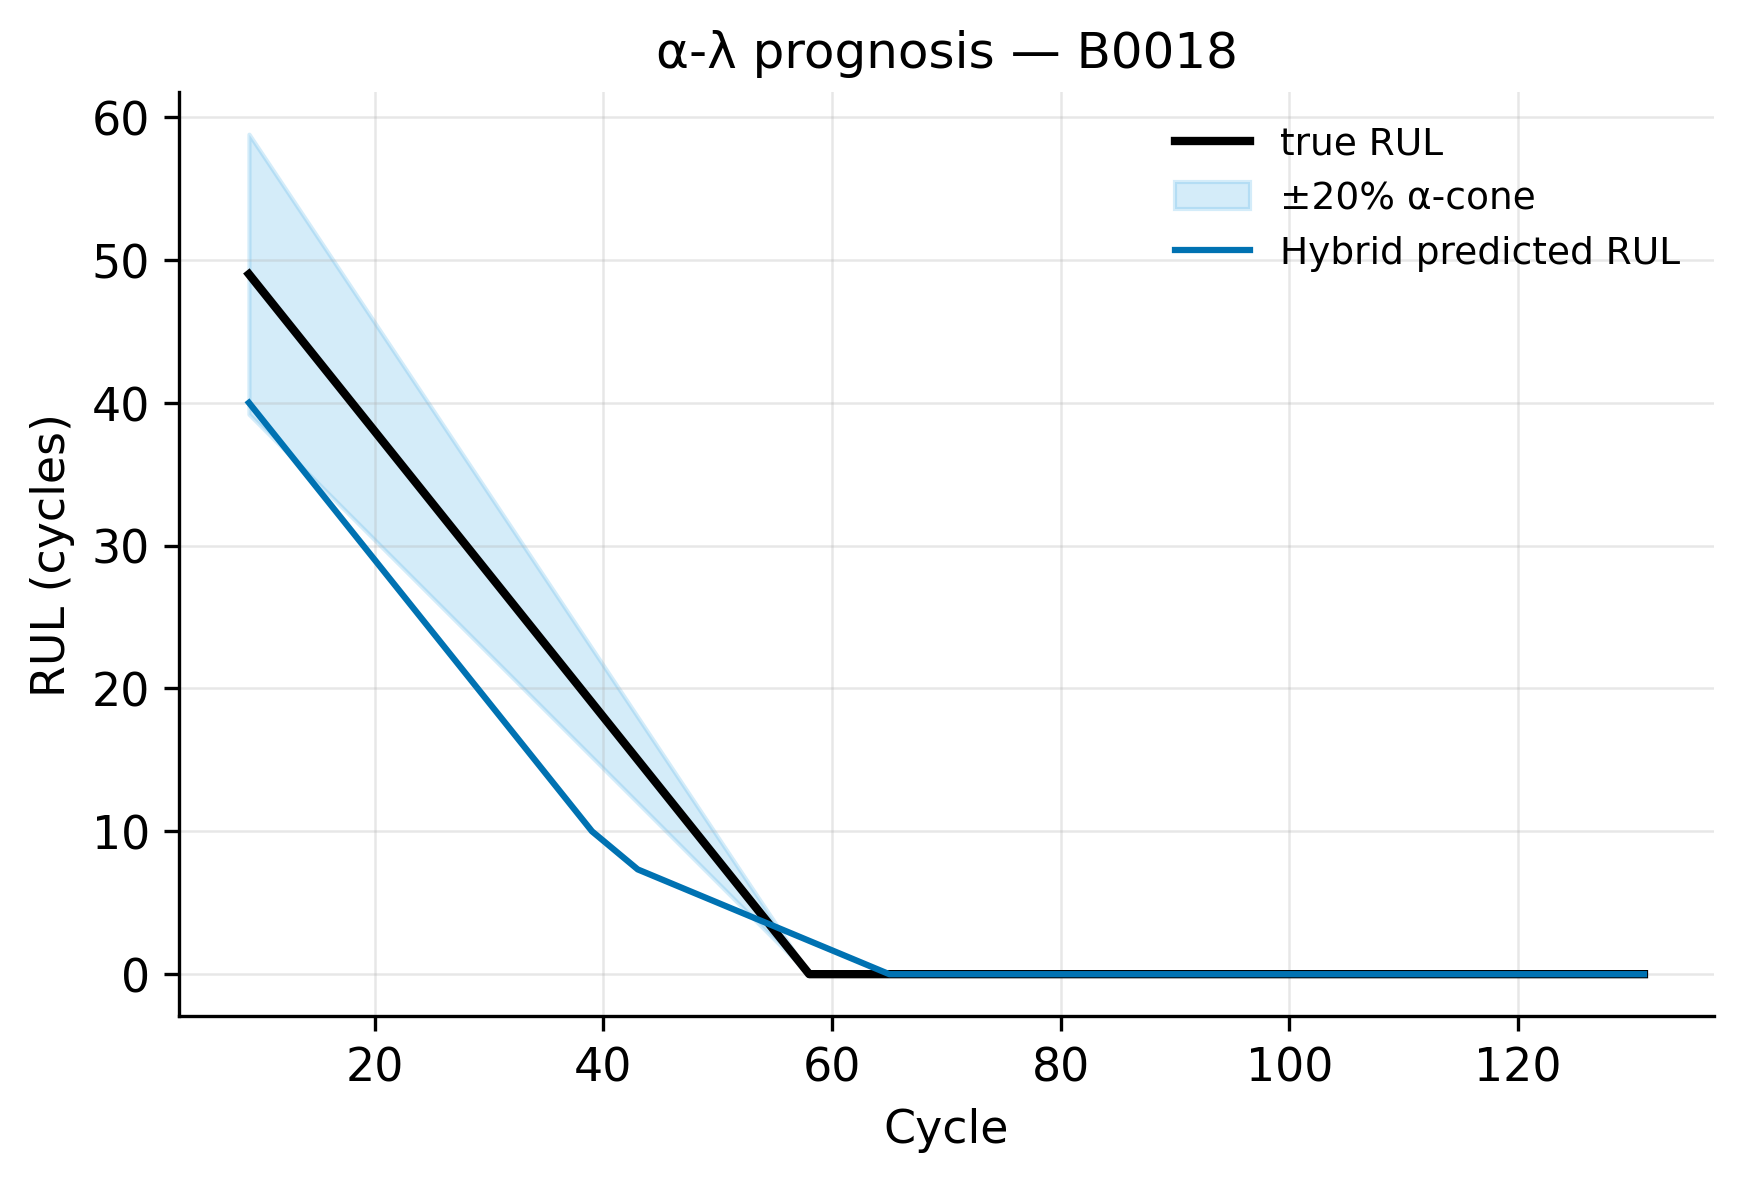
\includegraphics[width=0.80\textwidth]{2-mainmatter/chapters/alpha_lambda_B0018.png}
    \caption{$\alpha$-$\lambda$ RUL prognosis for the hybrid on the held-out cell
    B0018. The predicted RUL stays within (or close to) the $\pm20\%$ $\alpha$-cone
    through most of the cell's degradation, converging to the true end-of-life.}
    \label{fig:alpha_lambda}
\end{figure}

\begin{figure}[H]
    \centering
    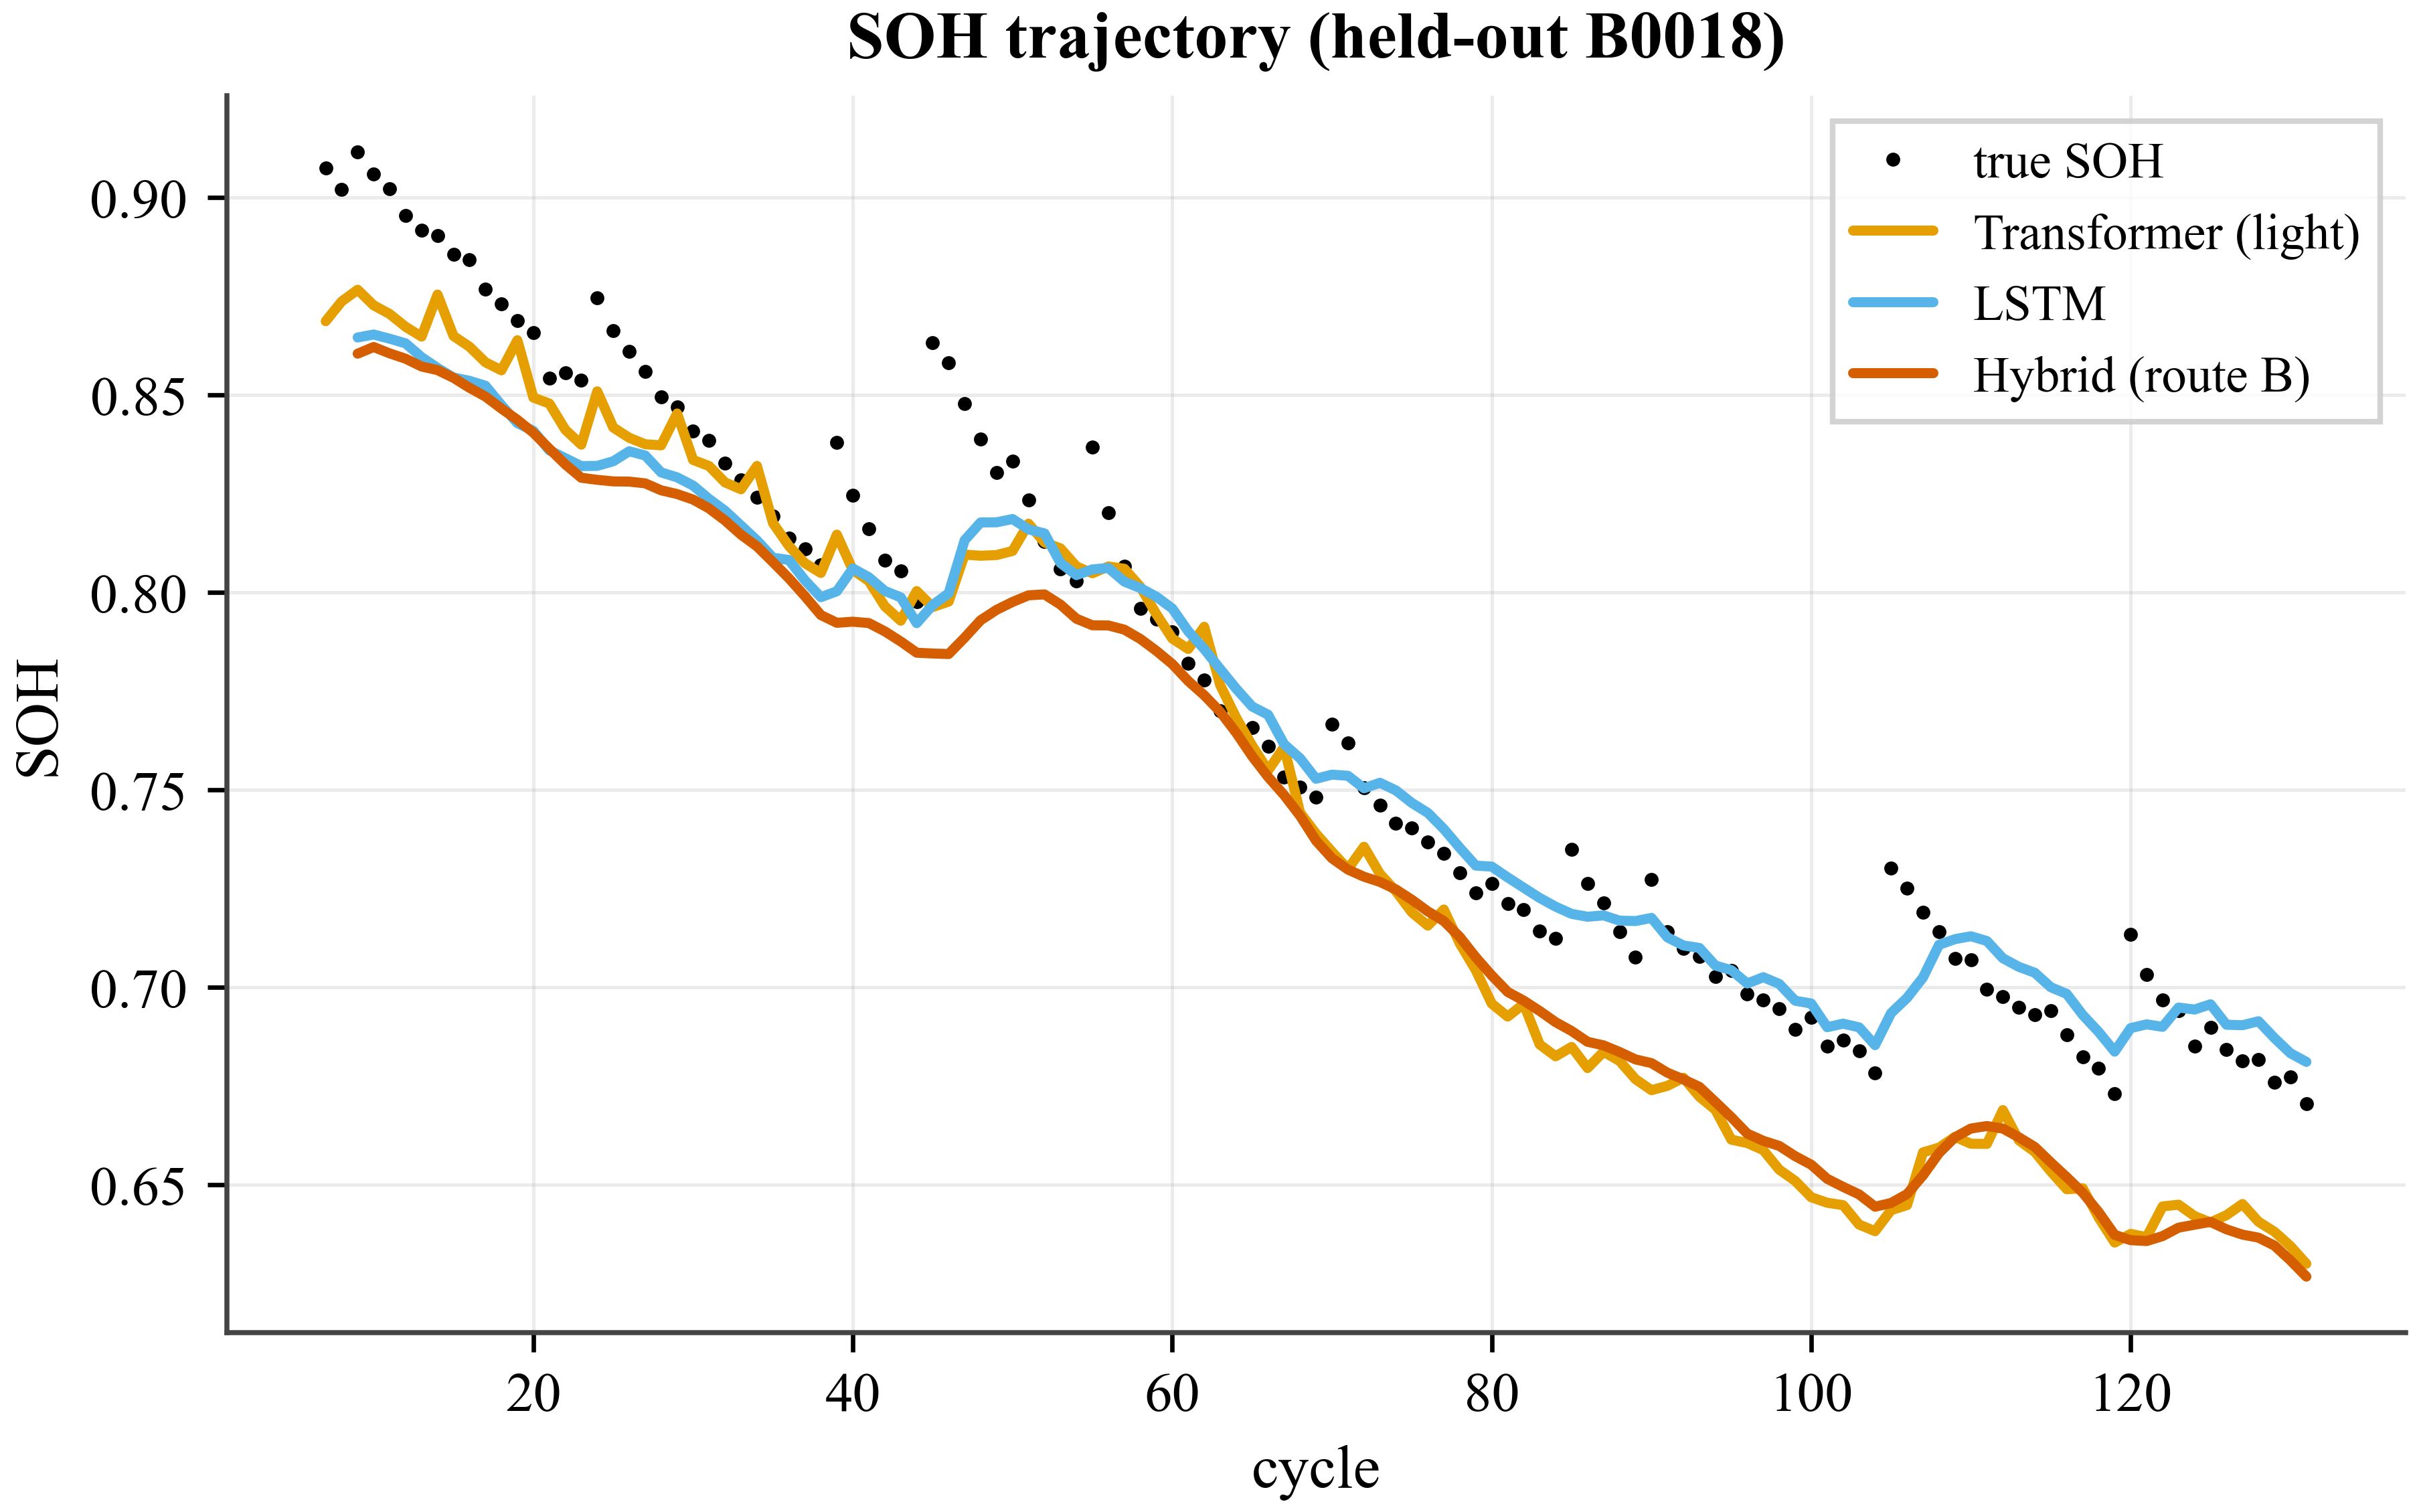
\includegraphics[width=0.80\textwidth]{2-mainmatter/chapters/soh_overlay_B0018.png}
    \caption{SOH trajectory on the held-out cell B0018. The hybrid follows the
    measured degradation trend without the phase lag visible in the purely
    data-driven baselines; consistent with its PCS lying above the ground-truth
    reference, it partially smooths the regeneration transients rather than
    reproducing every peak.}
    \label{fig:soh_b0018}
\end{figure}

\section{Ablation Studies}
\label{sec:ablations}

To isolate the contribution of each design choice, three ablations were run. The
design ablation (route / prior / weighting) uses 2 folds $\times$ 2 seeds for
speed; trends are consistent with the main benchmark, but absolute numbers are
indicative.

\begin{table}[H]
\centering
\caption{Physics-design ablation (route, prior, weighting), with a de-confound
control. ``Physics OFF $+$ t-channel'' has the route-B architecture (and thus the
extra cycle-coordinate input) but no ODE-residual penalty, isolating the input
feature from the physics.}
\label{tab:ablation}
\begin{tabular}{l c c c}
\toprule
\textbf{Variant} & \textbf{SOH RMSE} & \textbf{Phys.Cons.} & \textbf{Train (s)} \\
\midrule
Route B $\cdot$ ODE-residual (t $+$ physics) & \textbf{0.0251} & \textbf{0.909} & 3.26 \\
Physics OFF (no t, no physics)         & 0.0325 & 0.894 & 1.42 \\
Route A $\cdot$ double-exp             & 0.0343 & 0.891 & 1.59 \\
Physics OFF $+$ t-channel (control)    & 0.0367 & 0.903 & 3.07 \\
Route A $\cdot$ uncertainty-wt         & 0.0384 & 0.887 & 1.68 \\
Route A $\cdot$ logistic               & 0.0386 & 0.890 & 1.44 \\
\bottomrule
\end{tabular}
\end{table}

Four conclusions follow:
\begin{enumerate}
    \item \textbf{The de-confound control credits the physics, not the input.}
    Route~B's backbone takes the normalized cycle $t$ as an extra input, so a
    naive ``physics-off vs.\ route-B'' comparison would conflate the ODE loss
    with that feature. With the leak-free fixed-scale coordinate the control
    settles this cleanly: adding the $t$-channel \emph{alone} does not help
    (physics-off $0.0325 \rightarrow$ physics-off$+$t $0.0367$), while the ODE
    residual on top of the same architecture improves both accuracy
    ($0.0367 \rightarrow 0.0251$, also below the no-t baseline) and physical
    consistency ($0.903 \rightarrow 0.909$, the best of every variant). Under
    the earlier leaked normalization this control had pointed the other way
    (the coordinate itself carried test-cell information); with the corrected
    protocol the accuracy gain belongs to the physics term.
    \item \textbf{Route~B costs $\sim$2--3$\times$ the training time} of the
    no-physics baseline ($3.3$\,s vs.\ $1.4$\,s on this protocol). This training
    cost is paid offline; the deployed inference network is unchanged.
    \item \textbf{Uncertainty weighting did not have the impact we anticipated
    here.} On this small, clean problem the dynamic homoscedastic weighting did
    not improve on a well-chosen fixed weight ($0.0384$ vs.\ $0.0343$ for the same
    route-A backbone); the learned $\sigma$ tended to down-weight the data term
    more than was helpful. This refines the methodology of
    Chapter~\ref{ch:methodology}: the automatic weighting of Section~4.3 is a
    sound mechanism, but on a dataset of this size a carefully chosen fixed
    weight performs equally well (here slightly better), so the fixed weight is
    used for the headline models.
    \item \textbf{Within route~A the double-exponential prior beats the
    logistic} ($0.0343$ vs.\ $0.0386$), consistent with the AIC verdict of
    Table~\ref{tab:prior_fits}.
\end{enumerate}

\textbf{Aggregation ablation (feature richness).}
Table~\ref{tab:aggregation} compares the full 8-feature per-cycle representation
against a minimal 2-feature set. The richer representation gives a clear accuracy
gain ($0.0371$ vs.\ $0.0420$, $\approx12\%$): the ICA/DVA and
electrical-state features carry health information beyond a minimal
capacity summary. We note this is a \emph{feature-count} surrogate for the
per-second$\rightarrow$per-cycle trade-off rather than a literal comparison of
within-cycle sequence models against per-cycle scalars; a fuller study of
within-cycle representations is left as future work.

\begin{table}[H]
\centering
\caption{Aggregation ablation (route-A hybrid with double-exponential prior, mean
over 2 folds $\times$ 2 seeds).}
\label{tab:aggregation}
\begin{tabular}{l c c}
\toprule
\textbf{Feature set} & \textbf{SOH RMSE} & \textbf{Phys.Cons.} \\
\midrule
Full (8 features)    & \textbf{0.0371} & 0.895 \\
Minimal (2 features) & 0.0420 & \textbf{0.905} \\
\bottomrule
\end{tabular}
\end{table}

\textbf{Data-volume ablation.} Table~\ref{tab:datavolume} subsamples a stratified
fraction (25\%/50\%/75\%/100\%) of \emph{each} training cell's cycles for the
route-A hybrid (the inexpensive hybrid representative, as in the scarcity stress
test). The values sit in a $0.027$--$0.038$ band without a clean monotonic
trend; with two folds $\times$ two seeds the comparison is noise-dominated, and
the only cautious reading is that the hybrid does not collapse at low data
fractions. (An earlier version of this ablation kept the first $k\%$ of the
concatenated windows, which for small fractions was the early life of a single
cell; it was corrected to a per-cell stratified subsample so every training cell
remains represented.)

\begin{table}[H]
\centering
\caption{Data-volume ablation (route-A hybrid, stratified per-cell subsample, mean
over 2 folds $\times$ 2 seeds).}
\label{tab:datavolume}
\begin{tabular}{l c c}
\toprule
\textbf{Training data} & \textbf{SOH RMSE} & \textbf{Phys.Cons.} \\
\midrule
25\%  & 0.0375 & 0.891 \\
50\%  & 0.0338 & 0.894 \\
75\%  & 0.0369 & 0.892 \\
100\% & \textbf{0.0268} & 0.894 \\
\bottomrule
\end{tabular}
\end{table}

\section{Deployment Footprint (Cortex-M4)}
\label{sec:footprint}

A central claim of the thesis is that the framework is ``lightweight'' enough for
on-board BMS deployment. To make that claim on equal footing, a
\textbf{matched-size} route-B hybrid (hidden $=32$, $\approx$11k parameters,
comparable to the small GRU rather than the hidden-64 benchmark model) was
quantised to int8 and profiled against the Cortex-M4 budget (RAM $<256$\,KB,
flash $<1$\,MB, 80\,MHz). The footprint is reported in
Table~\ref{tab:footprint}.

\begin{table}[H]
\centering
\caption{Deployment footprint. Parameter counts, fp32 sizes, MACs, activation
RAM \emph{and int8 sizes} are measured on the trained models (int8 via PyTorch
dynamic quantisation with the qnnpack engine; linear and recurrent layers are
quantised, attention in-projections remain fp32, which is why the Transformers
compress by less than $4\times$). The Cortex-M4 latency is an analytic
MACs/clock (CMSIS-NN-style) estimate.}
\label{tab:footprint}
\small
\setlength{\tabcolsep}{3pt}
\begin{tabular}{l r r r r r c c}
\toprule
\textbf{Model} & \textbf{Params} & \textbf{fp32 (KB)} & \textbf{int8 (KB)} & \textbf{MACs} & \textbf{RAM (KB)} & \textbf{M4 lat.\ (ms)} & \textbf{Fits M4} \\
\midrule
Hybrid B (h=32) & 11{,}009 & 46.8 & \textbf{20.2} & 101{,}328 & \textbf{1.25} & 1.27 & yes \\
GRU (small)     &  4{,}161 & 18.6 & 9.2  & 39{,}392 & 1.25 & 0.49 & yes \\
Transformer (light) & 17{,}441 & 90.4 & 70.0 & 84{,}832 & 2.50 & 1.06 & yes \\
Transformer (heavy) & 225{,}409 & 932.1 & 611.1 & 1{,}114{,}656 & 7.50 & 13.93 & int8 only \\
\bottomrule
\end{tabular}
\end{table}

\begin{figure}[H]
    \centering
    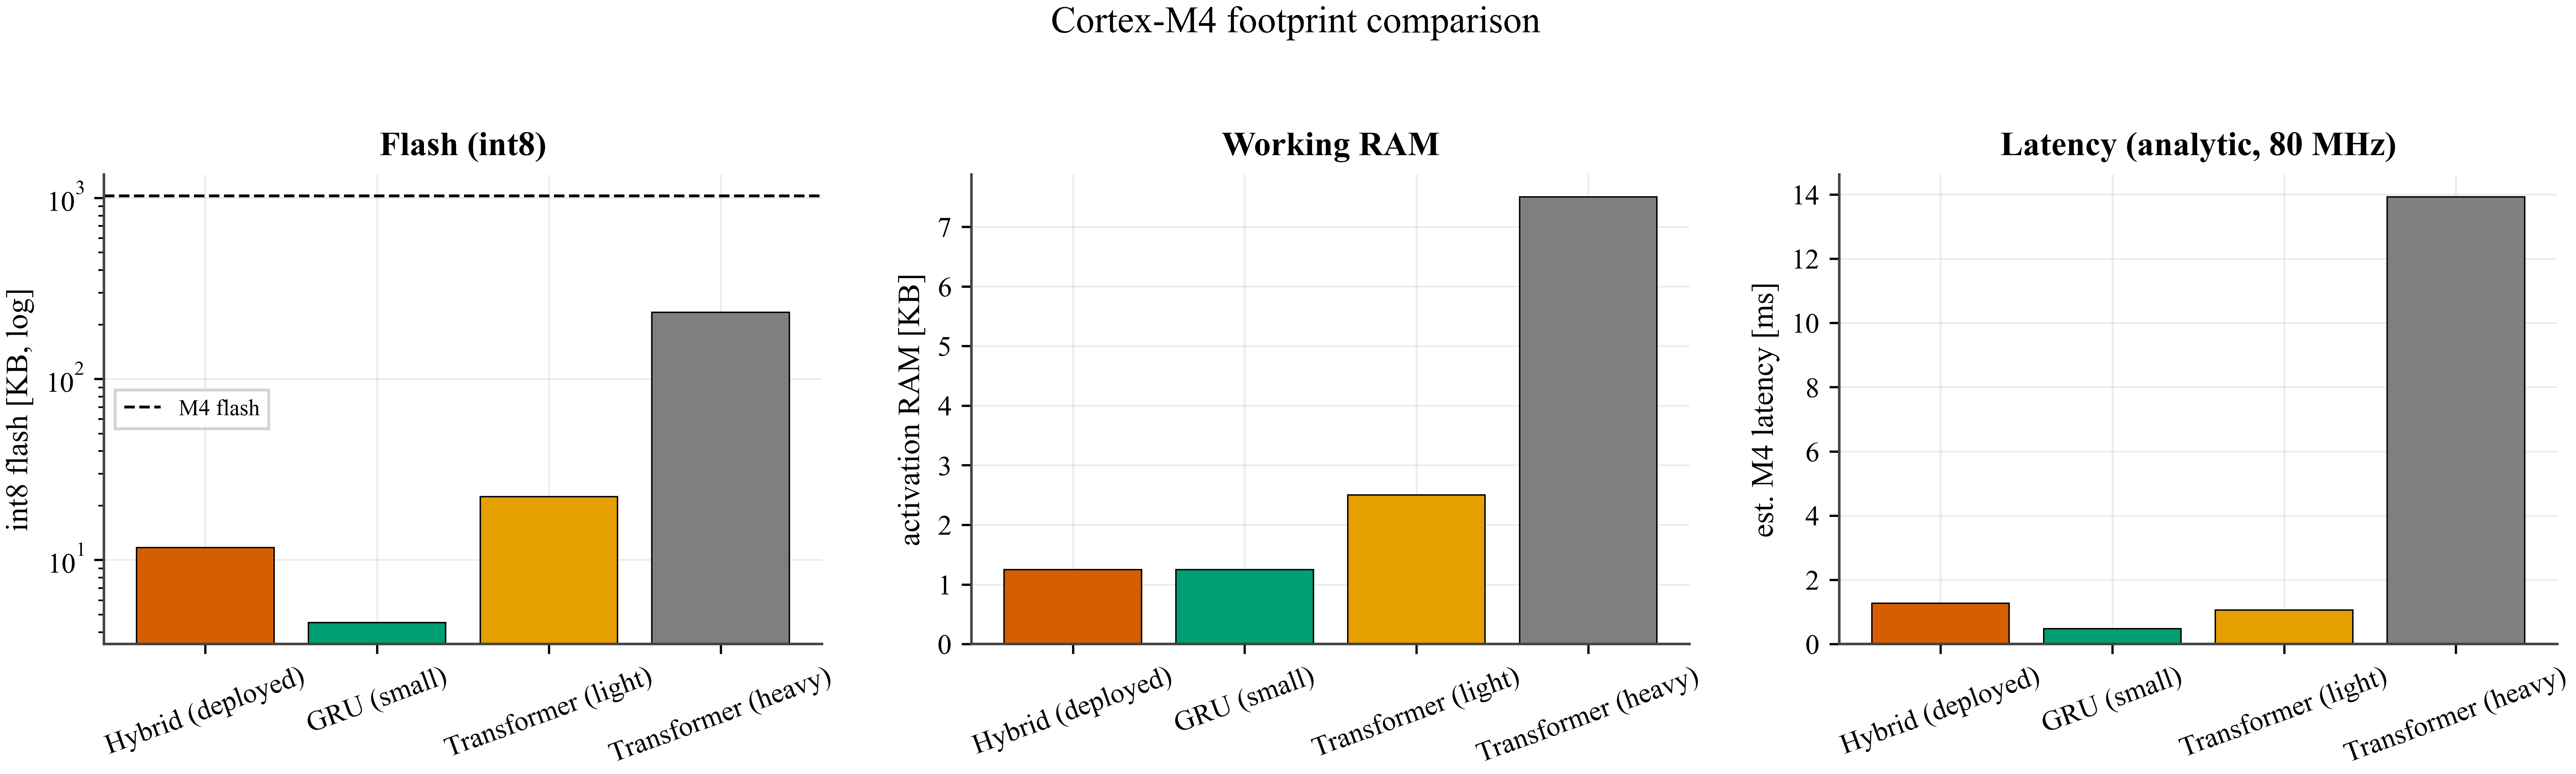
\includegraphics[width=1.0\textwidth]{2-mainmatter/chapters/footprint_comparison.png}
    \caption{Cortex-M4 footprint comparison: int8 flash (log scale, against the
    1\,MB budget), working RAM, and analytic latency at 80\,MHz. The deployable
    route-B hybrid needs $1/30$ the flash and $1/11$ the latency of the heavy
    Transformer, whose fp32 form (932\,KB) barely fits the flash budget at all
    and whose int8 form consumes 60\% of it.}
    \label{fig:footprint}
\end{figure}

The deployable hybrid occupies 20.2\,KB of measured int8 flash (2.0\% of the M4
budget) and 1.25\,KB of activation RAM. Evaluated on the same full four-fold
leave-one-cell-out protocol, it scores SOH RMSE $0.0328 \pm 0.0102$ with
physical consistency $0.893$: shrinking from 41k to 11k parameters costs some
accuracy ($0.0262 \rightarrow 0.0328$), but the deployed model still leads every
baseline in the benchmark --- it is more accurate than the heavy Transformer
($0.0418$) with $20\times$ fewer parameters, $30\times$ less flash, $6\times$
less RAM and $11\times$ lower estimated latency, and more accurate than the
light Transformer ($0.0345$) at $3.5\times$ less flash with better physical
consistency ($0.893$ vs.\ $0.783$). Figure~\ref{fig:frontier} summarises the
trade-off. Two methodological notes bound this result: the M4 latency is
analytic, not an on-board measurement, and the MAC counter instruments only the
linear and recurrent layers, so the Transformers' attention matrix products
($QK^\top$ and $AV$) are \emph{not} counted --- a bias in the Transformers'
favour, which makes the hybrid's reported latency advantage conservative.

\begin{figure}[H]
    \centering
    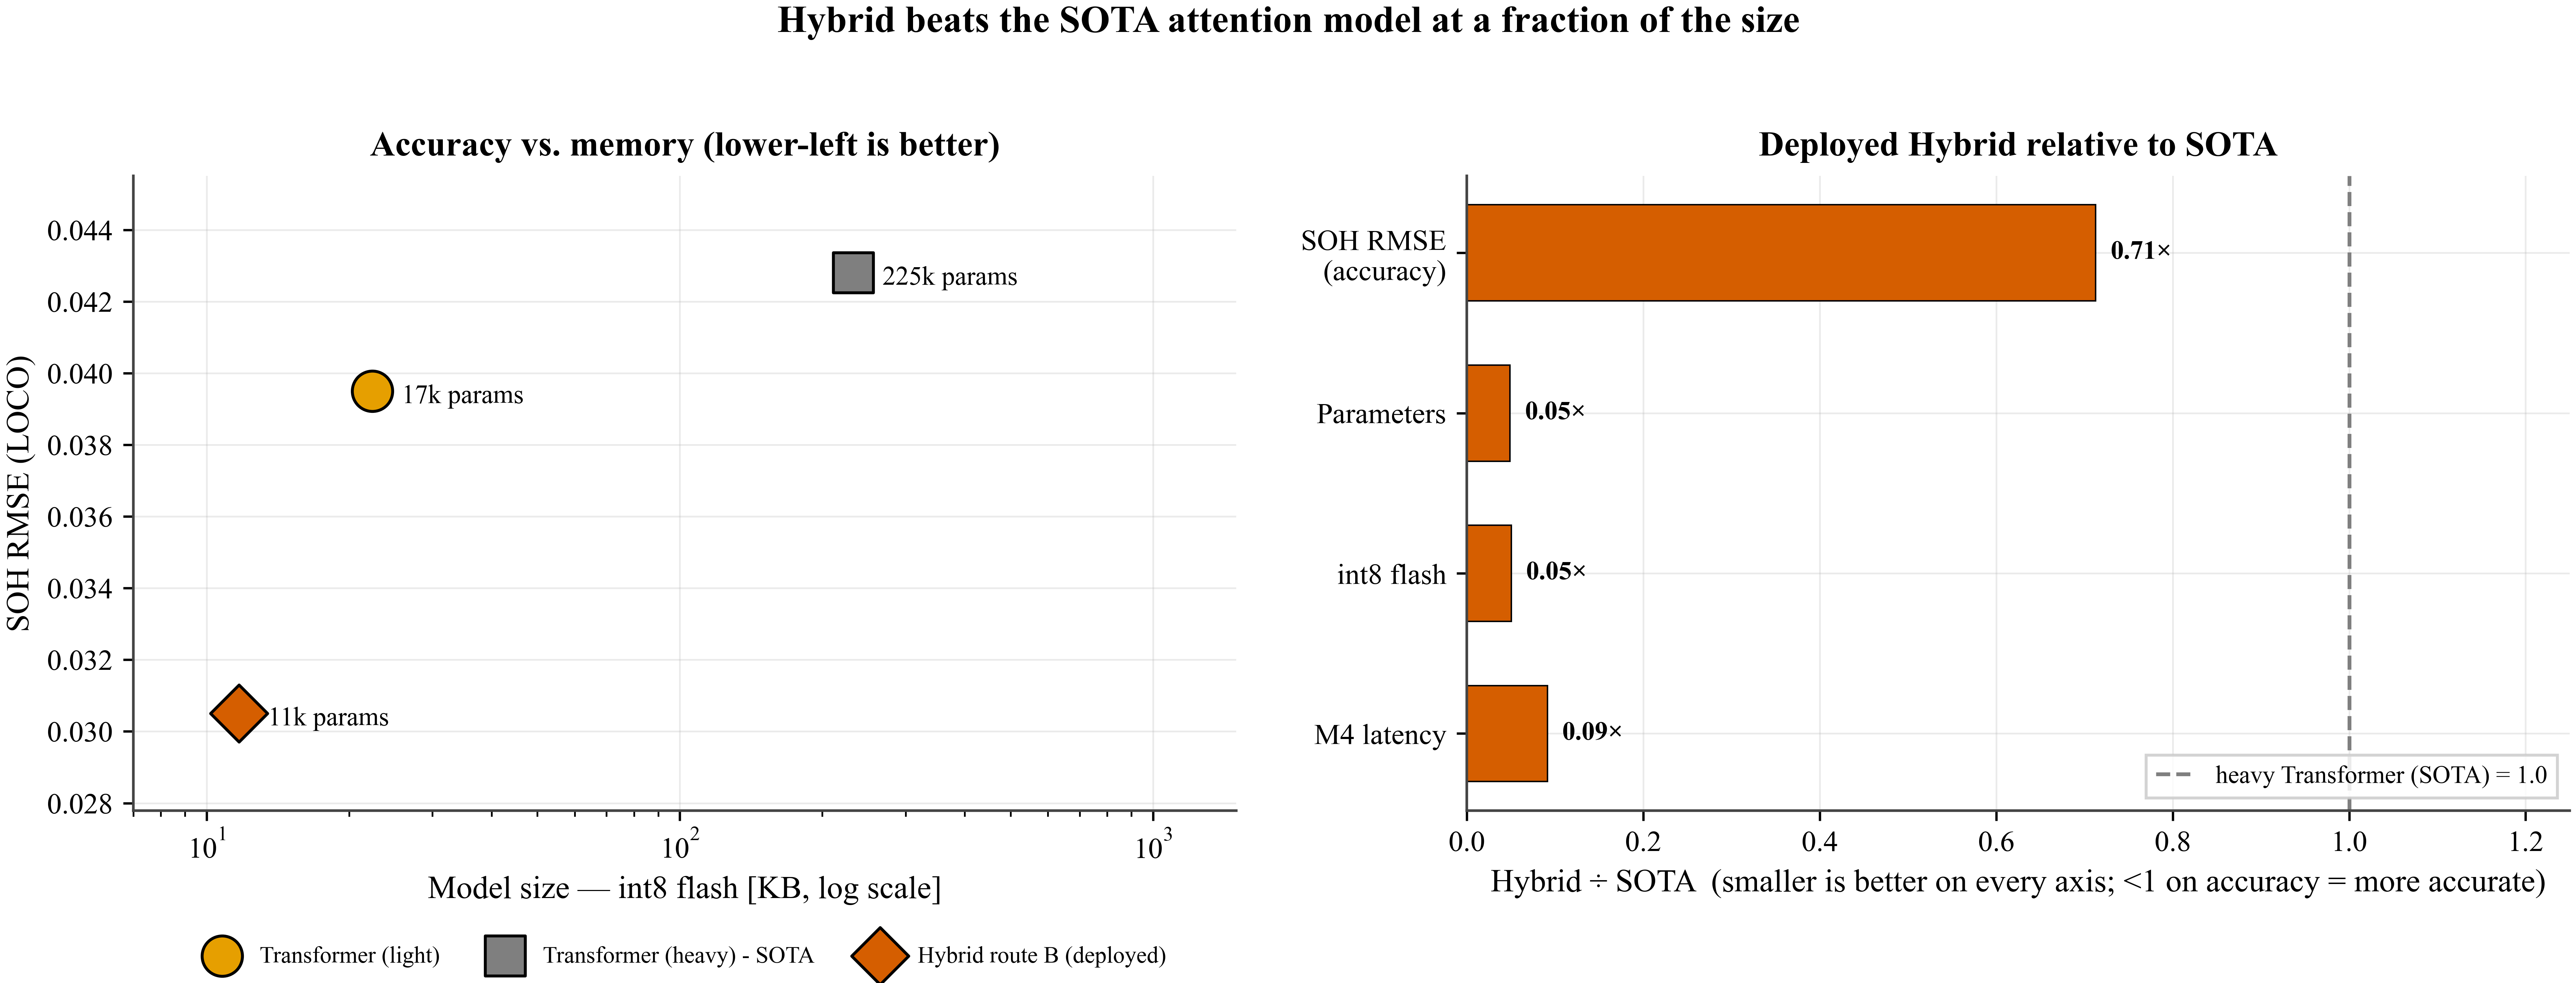
\includegraphics[width=1.0\textwidth]{2-mainmatter/chapters/frontier_vs_sota.png}
    \caption{The accuracy-vs-memory frontier. (Left) the deployed 11k-parameter
    hybrid occupies the favourable lower-left corner: more accurate than both
    Transformers at a fraction of the size. (Right) the deployed hybrid relative
    to the heavy Transformer on every axis.}
    \label{fig:frontier}
\end{figure}

\section{Implementation Caveats}
\label{sec:caveats}

For completeness, four implementation details that bound the claims are recorded
here rather than left implicit:

\begin{itemize}
    \item \textbf{Cycle-coordinate protocol.} An earlier draft normalized the
    cycle coordinate per trajectory, which leaked each test cell's total
    recorded life (the life fraction correlates with SOH at $|r|\ge0.97$). The
    corrected protocol uses a fixed scale ($\mathrm{cycle}/500$) supplied
    identically to every learned model; all results in this chapter use the
    corrected protocol. The residual limitation is extrapolation: on
    trajectories much longer than the training cells the coordinate leaves the
    training range, which is the mechanism behind route~B's cross-dataset
    degradation (Section~\ref{sec:cross_dataset}).
    \item \textbf{Quantisation and latency.} Int8 sizes are measured (dynamic
    quantisation, qnnpack engine); the M4 latency is analytic and conservative
    toward the Transformers, whose attention matrix products are excluded from
    the MAC count. On-board wall-clock measurement remains future work.
    \item \textbf{RUL persistence.} EOL \emph{labels} use the 5-cycle persistence
    rule of Chapter~\ref{ch:datasets_implementation}; the RUL curves derived
    from \emph{predicted} SOH trajectories at evaluation time use a 3-cycle
    persistence, a slightly more responsive setting applied identically to every
    model, so PHM comparisons between models are unaffected.
    \item \textbf{PHM metric coverage.} $\alpha$-$\lambda$, PH and CRA are
    computable only where both the true and the predicted trajectory cross the
    EOL threshold; folds where a model never predicts EOL drop out of that
    model's PHM average. This affects all models symmetrically but means the PHM
    columns average over slightly different fold subsets.
\end{itemize}

\section{Summary of Findings}
\label{sec:results_summary}

The measured evaluation supports the following conclusions:

\begin{itemize}
    \item \textbf{Learnable physics (route~B).} Under the leak-free, symmetric
    protocol the learnable ODE-residual is the most accurate model in the
    benchmark ($0.0262 \pm 0.0029$, the narrowest confidence interval), best or
    near-best on every unseen cell ($0.021$--$0.030$), the most physically
    consistent learned model ($0.918$), and the only learned model with
    clearly positive prognostic calibration (CRA $0.38$). The de-confound
    ablation attributes the gain to the ODE residual itself, not to the extra
    time input, which alone does not help.
    \item \textbf{Transformer comparison.} Attention models lead the literature
    on accuracy when trained on large corpora. At this data scale the
    high-capacity model is less accurate than the light one ($0.0418$ vs.\
    $0.0345$) and both trail the hybrid, which wins 11 of 12 runs against the
    heavy Transformer ($-37.5\%$ mean RMSE) and all 12 on physical consistency
    --- reported descriptively, since four independent cells cannot support
    formal significance.
    \item \textbf{Negative results, stated plainly.} The homoscedastic
    uncertainty weighting did not improve on a well-chosen fixed weight; the
    Neural-ODE baseline failed to clear the curve-fit floor; the data-volume and
    overfitting sweeps were noise-dominated at their reduced protocol; and
    route~B's cross-dataset transfer degrades ($0.2617$) because its cycle
    coordinate extrapolates outside the training range on the long-lived CALCE
    cell --- a failure the earlier leaked normalization had masked, with
    mitigations identified for future work.
    \item \textbf{Deployment.} The matched-size route-B hybrid requires a
    measured $20.2$\,KB of int8 flash (2.0\% of the Cortex-M4 budget) and
    $1.25$\,KB of RAM, and at that size ($0.0328$) it is still more accurate
    than every baseline --- $20\times$ fewer parameters, $30\times$ less flash
    and $11\times$ lower latency than the heavy Transformer, and $3.5\times$
    less flash than the light one with better accuracy and consistency.
\end{itemize}

These outcomes replace the interim report's claim that the hybrid always wins
with a more precise conclusion: a lightweight recurrent model with a learnable
physics regulariser is the best-balanced choice for deployable battery
prognostics in-distribution, a heavyweight attention model is neither small
enough for the edge nor more accurate at realistic data volumes, and the
framework's remaining weakness --- long-horizon extrapolation of the cycle
coordinate across datasets --- is identified, explained, and addressable.
